% --------------------------------------------------------------------------- %
% A0 paper poster for MetrumRG						   %
% --------------------------------------------------------------------------- %
% Created with Brian Amberg's LaTeX Poster Template. 					     %
% --------------------------------------------------------------------------- %

\documentclass[portrait,fontscale=0.3,paperwidth=36in,paperheight=48in]{baposter}

\usepackage{relsize}		% For \smaller
\usepackage{url}			% For \url
\usepackage{epstopdf}	% Included EPS files automatically converted to PDF to include with pdflatex

\usepackage[bitstream-charter]{mathdesign}
\usepackage[T1]{fontenc}

% Deprecating osfigures option; use oldstyle instead; 2020-09-10
\usepackage[defaultsans,oldstyle,scale=0.95]{opensans}

%%% Global Settings %%%%%%%%%%%%%%%%%%%%%%%%%%%%%%%%%%%%%%%%%%%%%%%%%%%%%%%%%%%

\graphicspath{{pix/}}	% Root directory of the pictures 
\tracingstats=2			% Enabled LaTeX logging with conditionals

%%% Color Definitions %%%%%%%%%%%%%%%%%%%%%%%%%%%%%%%%%%%%%%%%%%%%%%%%%%%%%%%%%

\definecolor{bordercol}{RGB}{40,40,40}
\definecolor{headercol1}{RGB}{186,215,230}
\definecolor{headercol2}{RGB}{80,80,80}
\definecolor{headerfontcol}{RGB}{0,0,0}
\definecolor{boxcolor}{RGB}{186,215,230}
\definecolor{metgreen}{rgb}{0,0.555,0}
\definecolor{lightergreen}{rgb}{.8,1,0.85}
\definecolor{lightergray}{RGB}{225,225,225}
\definecolor{darkteal}{RGB}{41, 127, 157}
\definecolor{tealdark}{RGB}{41, 104, 157}
\definecolor{red}{RGB}{180, 55, 87}

%%% Metrum's official green RGB is weirdly greyish-green so using
% the green below to get a close match to the Metrum M
\definecolor{Mgreen}{RGB}{0, 120,  50}

% Macro's to include text in metrums green, in bold or italics
% Can be useful to subtly draw the readers eye
\newcommand{\greenBF}[1]{\textcolor{Mgreen}{\textbf{#1}}}
\newcommand{\greenIT}[1]{\textcolor{Mgreen}{\textit{#1 }}}

%% Use this to put a box around a specific section, within an existing higher level box
%% E.g., to split the results box into sub-sections if desired. 
%% See FOCE example project poster for examples 
%% https://ghe.metrumrg.com/example-projects/bbr-nonmem-poppk-foce/blob/main/deliv/poster-acop-2022/acop13-expo-poster-final.pdf
\usepackage{tcolorbox}
\newtcolorbox{demobx}[1][]{colback=white,colframe=Mgreen,width=0.98\linewidth,nobeforeafter,box align=top,before=\noindent,#1}



% PLEASE MODIFY COLOR SCHEME HERE IF NEEDED
\colorlet{titlefgcol}{black}
\colorlet{headerbgcol}{Mgreen}
\colorlet{headerfgcol}{white}
\colorlet{bordercol}{lightergray}
\newcommand{\headershade}{none}

%%%%%%%%%%%%%%%%%%%%%%%%%%%%%%%%%%%%%%%%%%%%%%%%%%%%%%%%%%%%%%%%%%%%%%%%%%%%%%%%
%%% Utility functions %%%%%%%%%%%%%%%%%%%%%%%%%%%%%%%%%%%%%%%%%%%%%%%%%%%%%%%%%%

%%% Save space in lists. Use this after the opening of the list %%%%%%%%%%%%%%%%
\newcommand{\compresslist}{
	\setlength{\itemsep}{1pt}
	\setlength{\parskip}{0pt}
	\setlength{\parsep}{0pt}
}

%%%%%%%%%%%%%%%%%%%%%%%%%%%%%%%%%%%%%%%%%%%%%%%%%%%%%%%%%%%%%%%%%%%%%%%%%%%%%%%
%%% Document Start %%%%%%%%%%%%%%%%%%%%%%%%%%%%%%%%%%%%%%%%%%%%%%%%%%%%%%%%%%%%
%%%%%%%%%%%%%%%%%%%%%%%%%%%%%%%%%%%%%%%%%%%%%%%%%%%%%%%%%%%%%%%%%%%%%%%%%%%%%%%

\begin{document}
\typeout{Poster rendering started}

%%% Setting Background Image %%%%%%%%%%%%%%%%%%%%%%%%%%%%%%%%%%%%%%%%%%%%%%%%%%
\background{
%	\begin{tikzpicture}[remember picture,overlay]%
%	\draw (current page.north west)+(-2em,2em) node[anchor=north west]
%	{\includegraphics[height=1.1\textheight]{background}};
%	\end{tikzpicture}
}

%%% General Poster Settings %%%%%%%%%%%%%%%%%%%%%%%%%%%%%%%%%%%%%%%%%%%%%%%%%%%
%%%%%% Eye Catcher, Title, Authors and University Images %%%%%%%%%%%%%%%%%%%%%%
\begin{poster}{
	grid=false,
	% Option is left on true though the eyecatcher is not used. The reason is
	% that we have a bit nicer looking title and author formatting in the headercol
	% this way
	columns = 3,
	eyecatcher=false, 
	borderColor=bordercol,
	headerColorOne=headerbgcol,
	headerColorTwo=headerbgcol,
	headerFontColor=headerfgcol,
	% Only simple background color used, no shading, so boxColorTwo isn't necessary
	boxColorOne=white,
	headershape=rectangle,
	headerfont=\Large\bf\textsf,
	textborder=rectangle,
	background=user,
	headerborder=open,
  boxshade=none, 
  headershade=plain,
  headerheight=0.116\textheight %% CHANGE THIS TO INCREASE ROOM FOR LONG TITLE
}
%%% Eye Cacther %%%%%%%%%%%%%%%%%%%%%%%%%%%%%%%%%%%%%%%%%%%%%%%%%%%%%%%%%%%%%%%
{
%	Eye Catcher, empty if option eyecatcher=false - unused
}
%%% Title %%%%%%%%%%%%%%%%%%%%%%%%%%%%%%%%%%%%%%%%%%%%%%%%%%%%%%%%%%%%%%%%%%%%%
{\smaller
	\textbf{\textsf{\color{titlefgcol}{ 
		Towards the development of a platform PBPK-QSP model in the Julia programming language for evaluating potential toxicities caused by antibody-drug-conjugate therapies
	 }}}\vspace{.5em}
}
%%% Authors %%%%%%%%%%%%%%%%%%%%%%%%%%%%%%%%%%%%%%%%%%%%%%%%%%%%%%%%%%%%%%%%%%%
{\smaller  \smaller 
	Yuezhe Li$^1$, A. Katharina Wilkins$^1$  \\
	{\smaller  
	  $^1$\textit{Metrum Research Group, Tariffville, CT}
	}
}
%%% Logo %%%%%%%%%%%%%%%%%%%%%%%%%%%%%%%%%%%%%%%%%%%%%%%%%%%%%%%%%%%%%%%%%%%%%%
{
% The logos are compressed a bit into a simple box to make them smaller on the result
% (Wasn't able to find any bigger of them.)
%\setlength\fboxsep{5pt}
%\setlength\fboxrule{0.5pt}
%	\fbox{
		\begin{minipage}{16em}
			\begin{center}
			
\includegraphics[width=14em]{newlogo} 
			\end{center}
		\end{minipage}
%	}
}
%%%%%%%%%%%%%%%%%%%%%%%%%%%%%%%%%%%%%%%%%%%%%%%%%%%%%%%%%%%%%%%%%%%%%%%%%%%%%%%%
%%%%%%%%%%%%%%%%%%%%%%%%%%%%%%%%%%%%%%%%%%%%%%%%%%%%%%%%%%%%%%%%%%%%%%%%%%%%%%%%


\headerbox{Abstract}{name=abstract,column=0,row=0}{
\footnotesize 

Antibody-drug-conjugates (ADCs) are a rapidly expanding class of anti-cancer drugs. 
They were developed with the aim to expand the therapeutic index of potent cytotoxic agents (i.e., payload) by employing the targeting specificity of monoclonal antibodies (mAbs) to direct the delivery of payload selectively to malignant cells. 
Although many ADCs have demonstrated efficacy, their clinical use tends to lead to substantial, sometimes dose-limiting toxicities. 
Moreover, promising candidate ADCs continue to fail late in the development pipeline, after demonstrating activity in preclinical studies, because their toxicity profiles prevent dosing at levels high enough to achieve clinical efficacy. 

Here, a physiologically based pharmacokinetics (PBPK) - quantitative systems pharmacology (QSP) model to predict both off- and on-target off-tumor toxicities of ADCs was developed by combining published models. 
This model could predict the observed liver and lung toxicity of trastuzumab emtansine (T-DM1), a widely used ADC to treat HER-2 positive breast cancer. 
It also predicted the low hepatotoxicity of trastuzumab deruxtecan (T-Dxd), another HER-2 targeting ADC, and brentuximab vedotin (BV), an ADC used to treat lymphoma. 
Furthermore, this model could predict the high hepatotoxicity observed in cantuzumab mertansine (CM), an ADC suspended from development.

}
%%%%%%%%%%%%%%%%%%%%%%%%%%%%%%%%%%%%%%%%%%%%%%%%%%%%%%%%%%%%%%%%%%%%%%%%%%%%%%%%
%%%%%%%%%%%%%%%%%%%%%%%%%%%%%%%%%%%%%%%%%%%%%%%%%%%%%%%%%%%%%%%%%%%%%%%%%%%%%%%%


\headerbox{Methods}{name=methods,column=0,below=abstract}{
\footnotesize 

The systemic pharmacokinetics (PK) of ADCs were described by a previously published PBPK model [1] (Fig 1A). 
Plasma ADC could bound to soluble receptor and being degraded (Fig 1C).
For the ADC that were not degraded, they could either enter tissue endothelial cells through either FcRn-mediated or FcRn-independent processes before reaching the tissue interstitium (Fig 1B), or into tumor through vascular and surface exchange [2] (Fig 1A). 
For those reached tissue interstitium (including tumor interstitium),  they could enter cells through receptor-mediated uptake [3] (Fig 1A). 
ADC inside cells (endothelial cells and tumor cells) could be degraded and release payload, inducing cell killing. 

\begin{minipage}{\textwidth}
\centering
	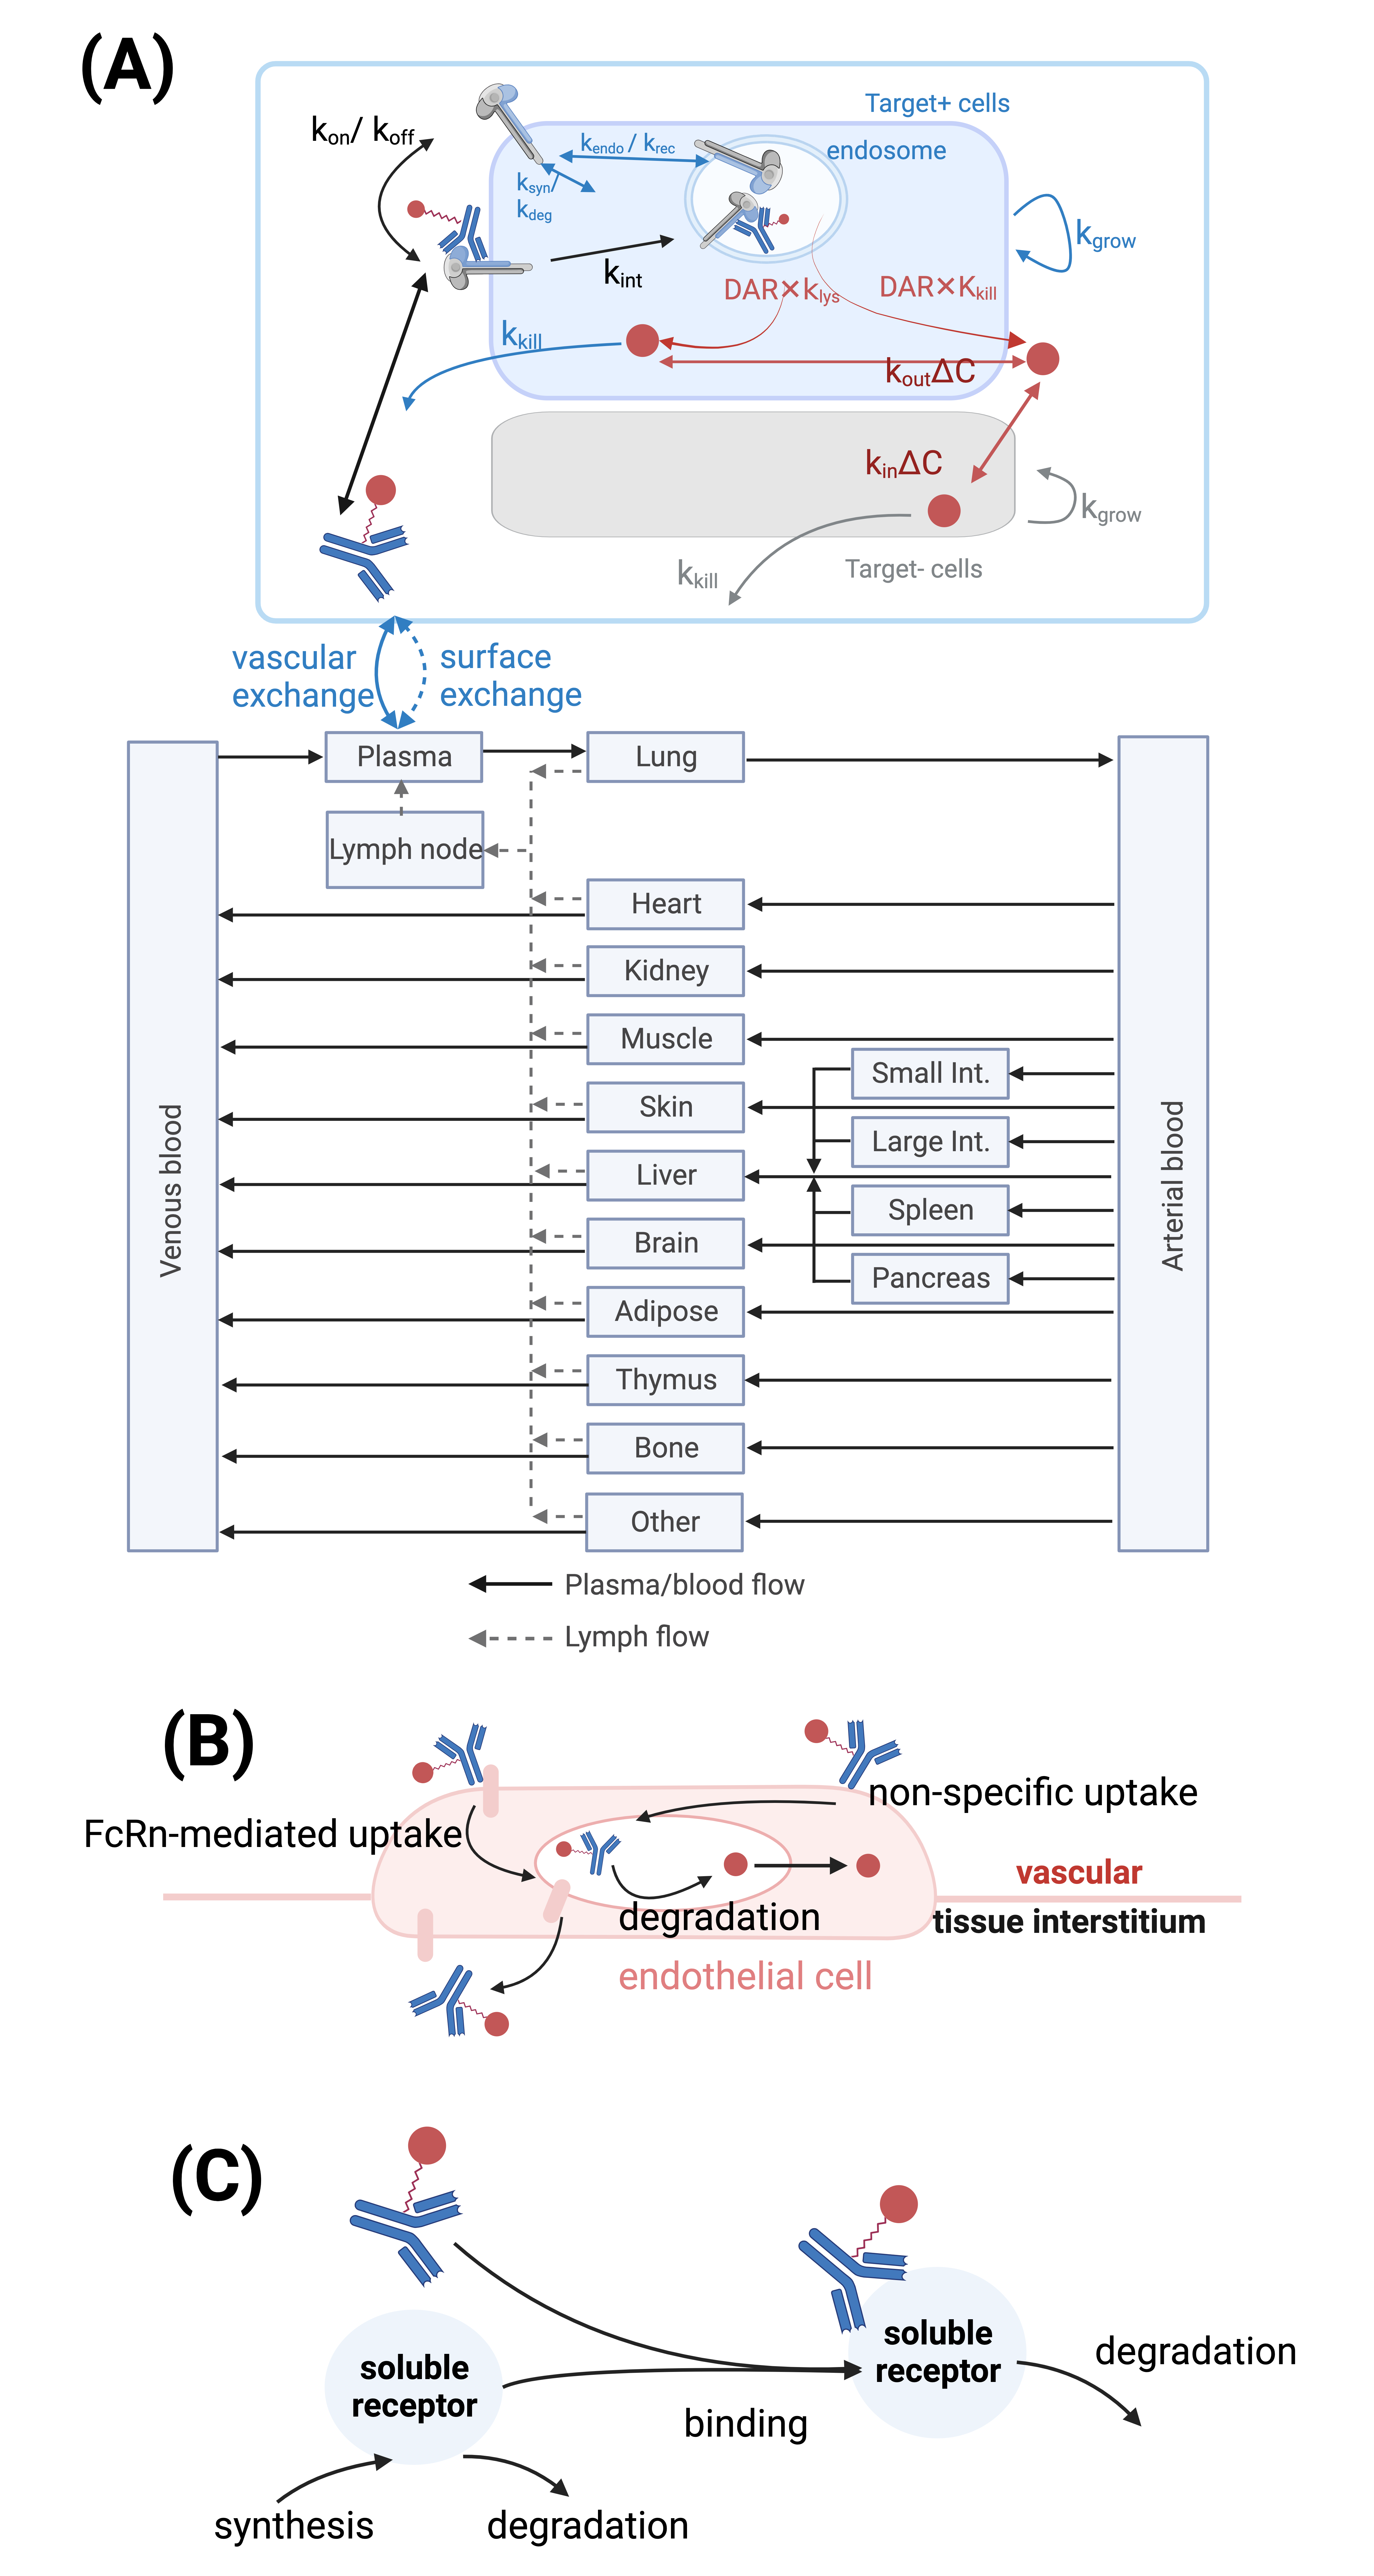
\includegraphics[width= 0.98 \textwidth]{../img/adc-distribution-diagram}

\scriptsize{\textbf{Fig 1}. (A) PBPK model for ADC distribution across the system and QSP model for ADC PD model in tumor. 
		(B) ADC uptake and payload dynamics in tissue endothelial cells. (C) Dynamics of ADC and soluble receptor in plasma. }
\end{minipage}

}



%%%%%%%%%%%%%%%%%%%%%%%%%%%%%%%%%%%%%%%%%%%%%%%%%%%%%%%%%%%%%%%%%%%%%%%%%%%%%%%%
%%%%%%%%%%%%%%%%%%%%%%%%%%%%%%%%%%%%%%%%%%%%%%%%%%%%%%%%%%%%%%%%%%%%%%%%%%%%%%%%


\headerbox{Results}{name=results,span=2,column=1,row=0}{
\footnotesize

ADCs included in this study were listed in Table 1. The model was calibrated using their PK profiles (Fig 2A-D). 

\begin{minipage}[b]{0.24\linewidth}
\centering
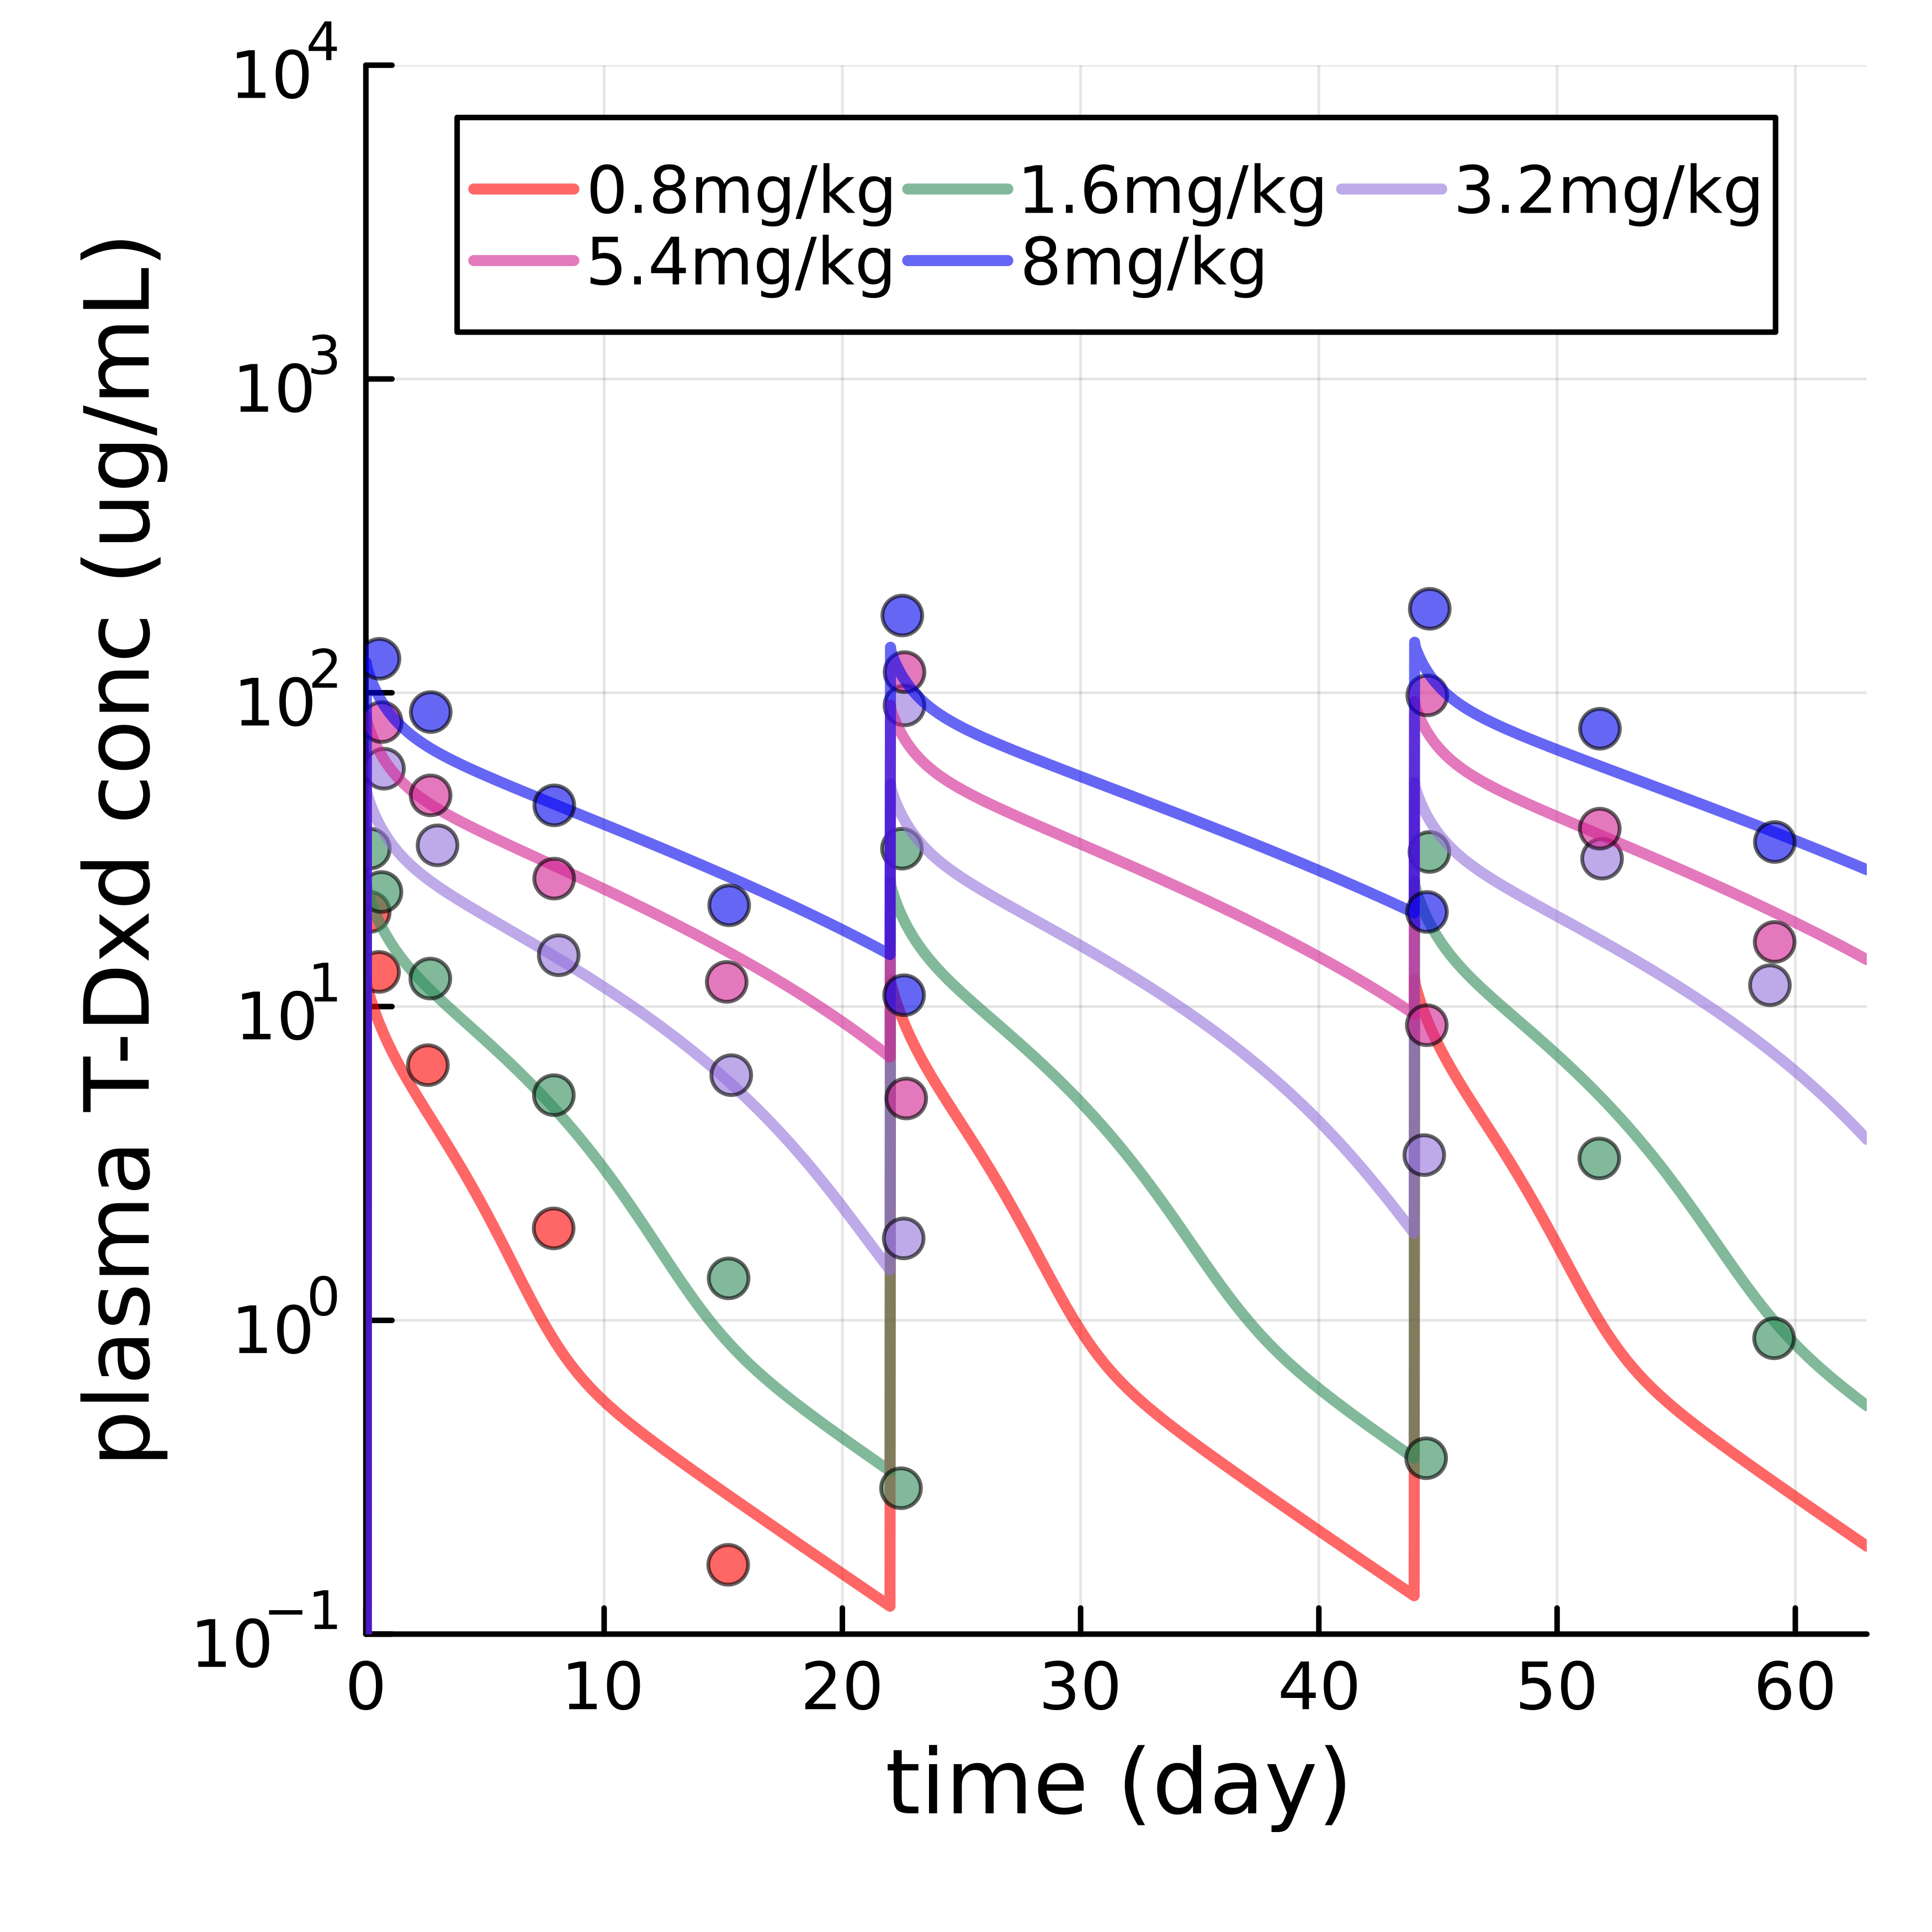
\includegraphics[width=\textwidth]{../img/t-dxd-pk.png}
\scriptsize{Fig 2A. T-Dxd PK. (data source [4])}
\end{minipage}
\begin{minipage}[b]{0.24\linewidth}
\centering
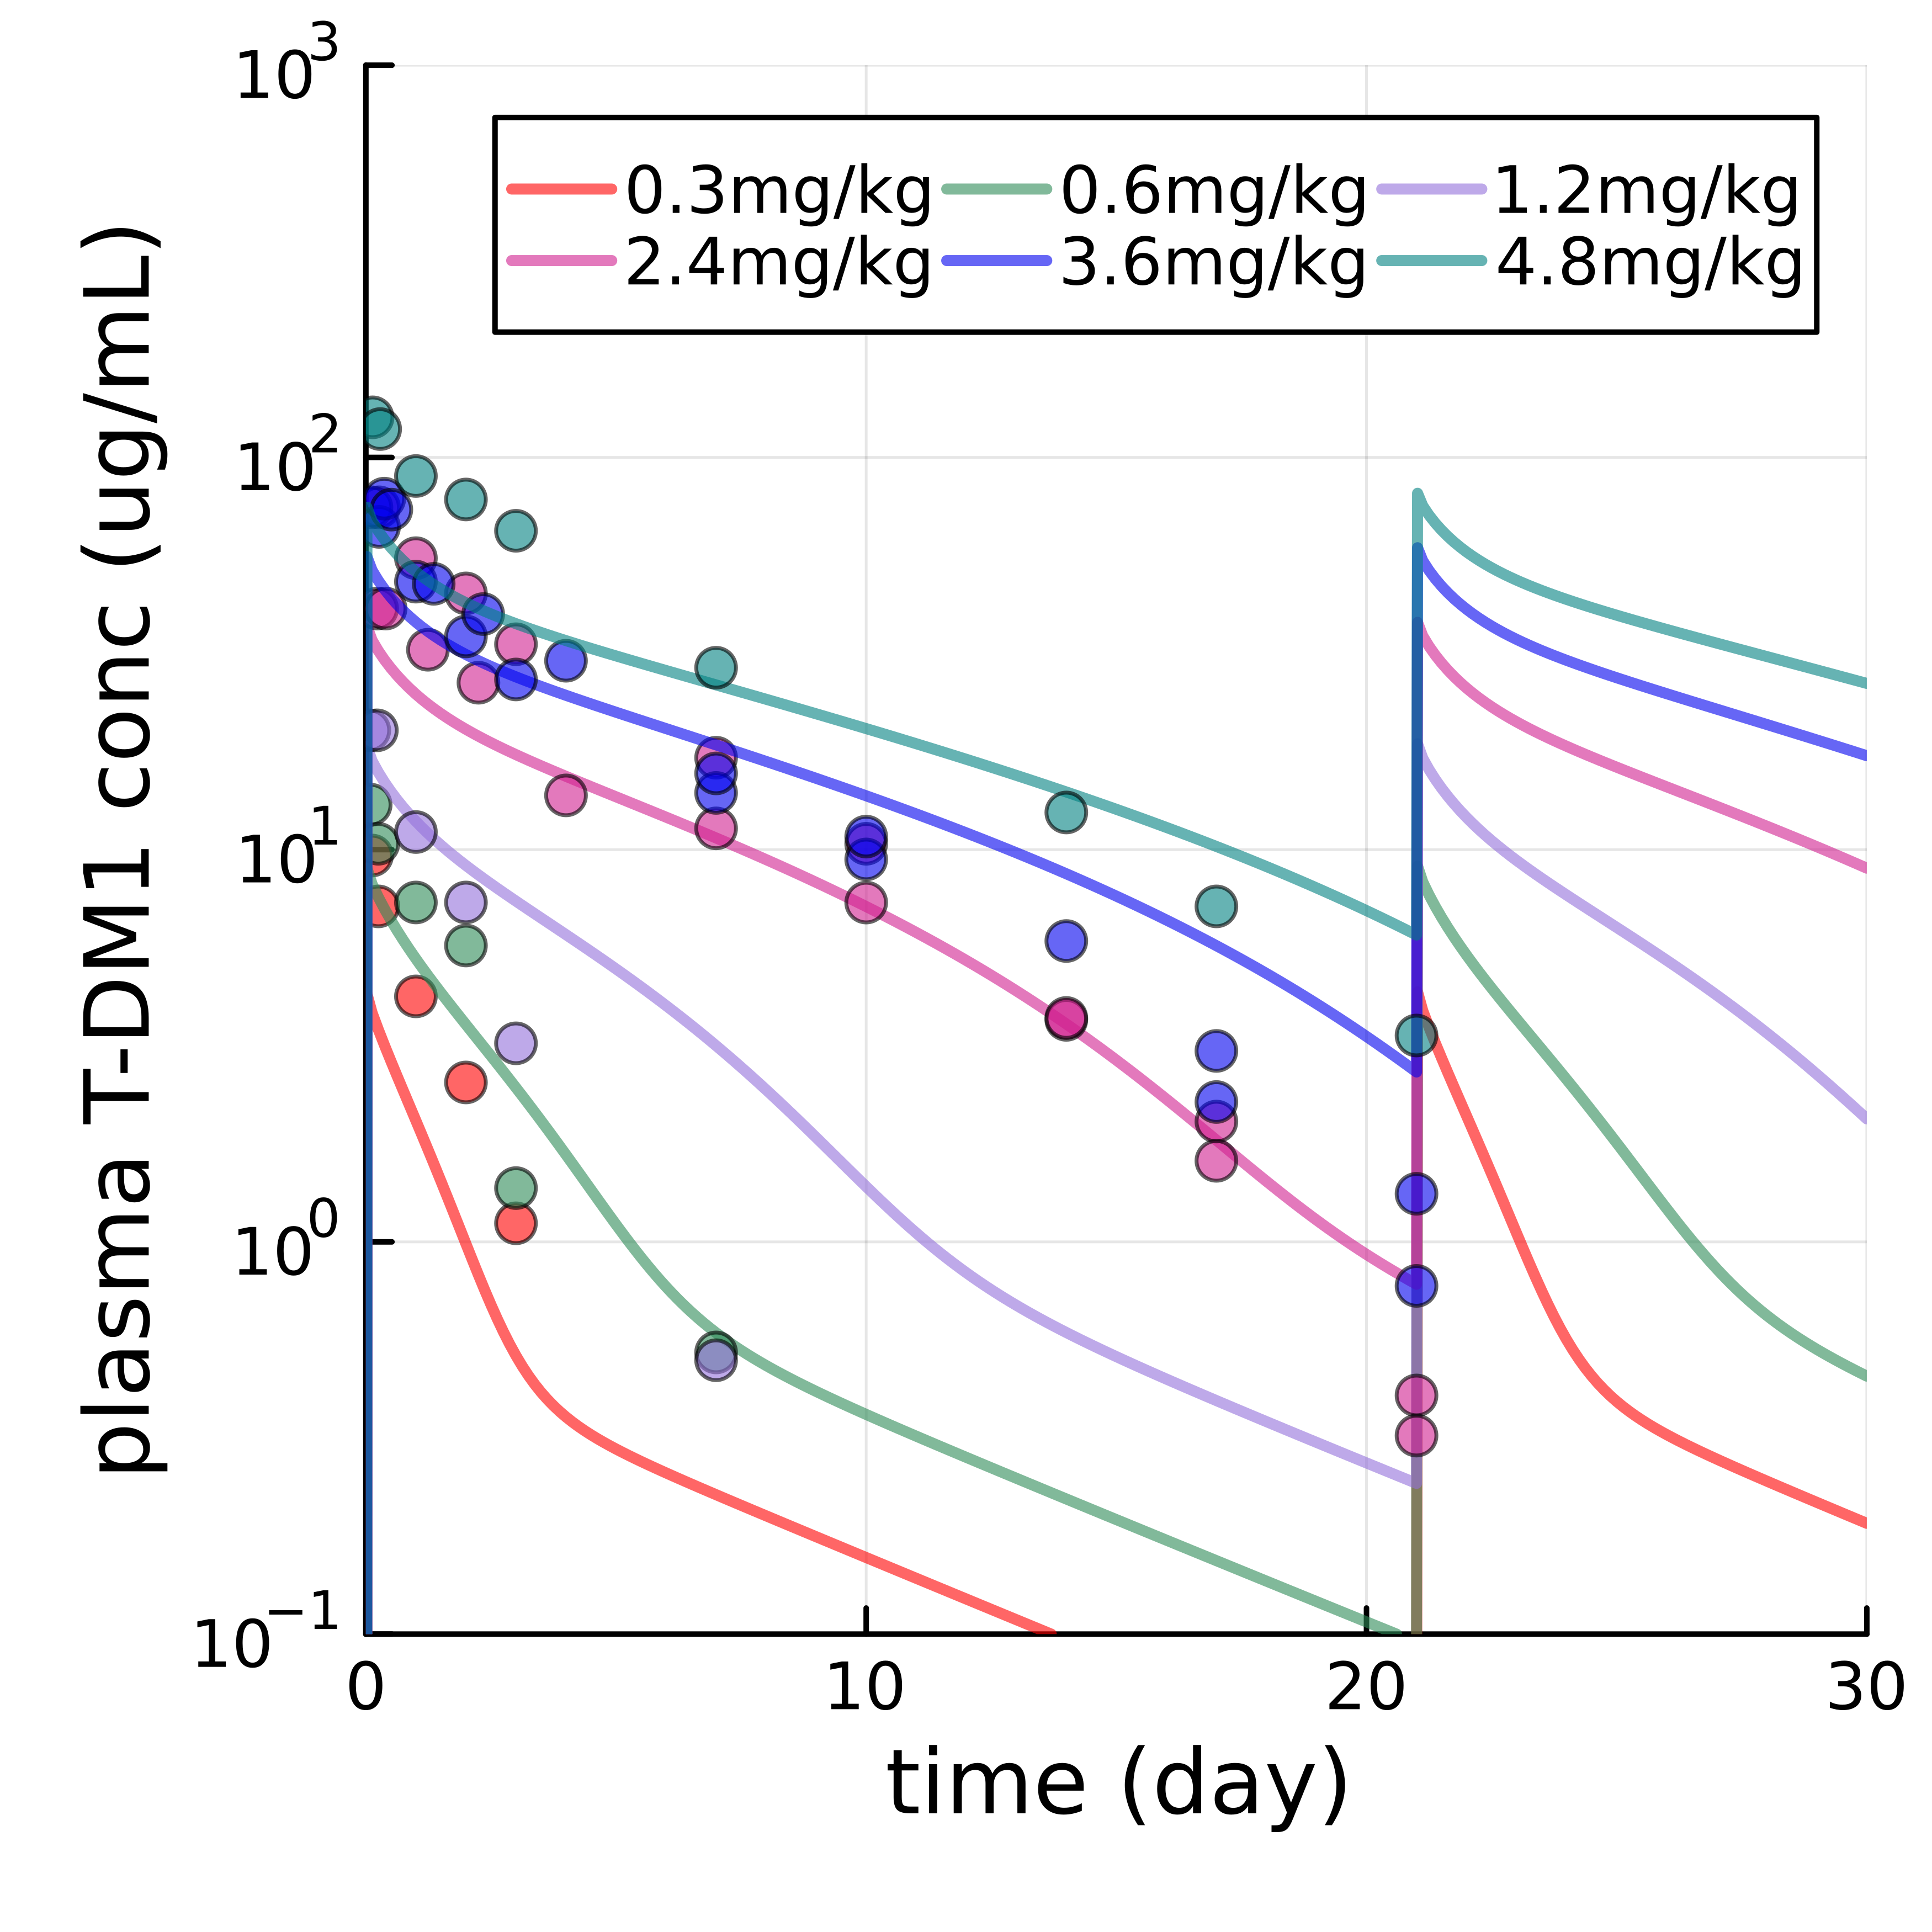
\includegraphics[width=\textwidth]{../img/t-dm1-pk.png}
\scriptsize{Fig 2B. T-DM1 PK. (data source [5])}
\end{minipage}
\begin{minipage}[b]{0.24\linewidth}
\centering
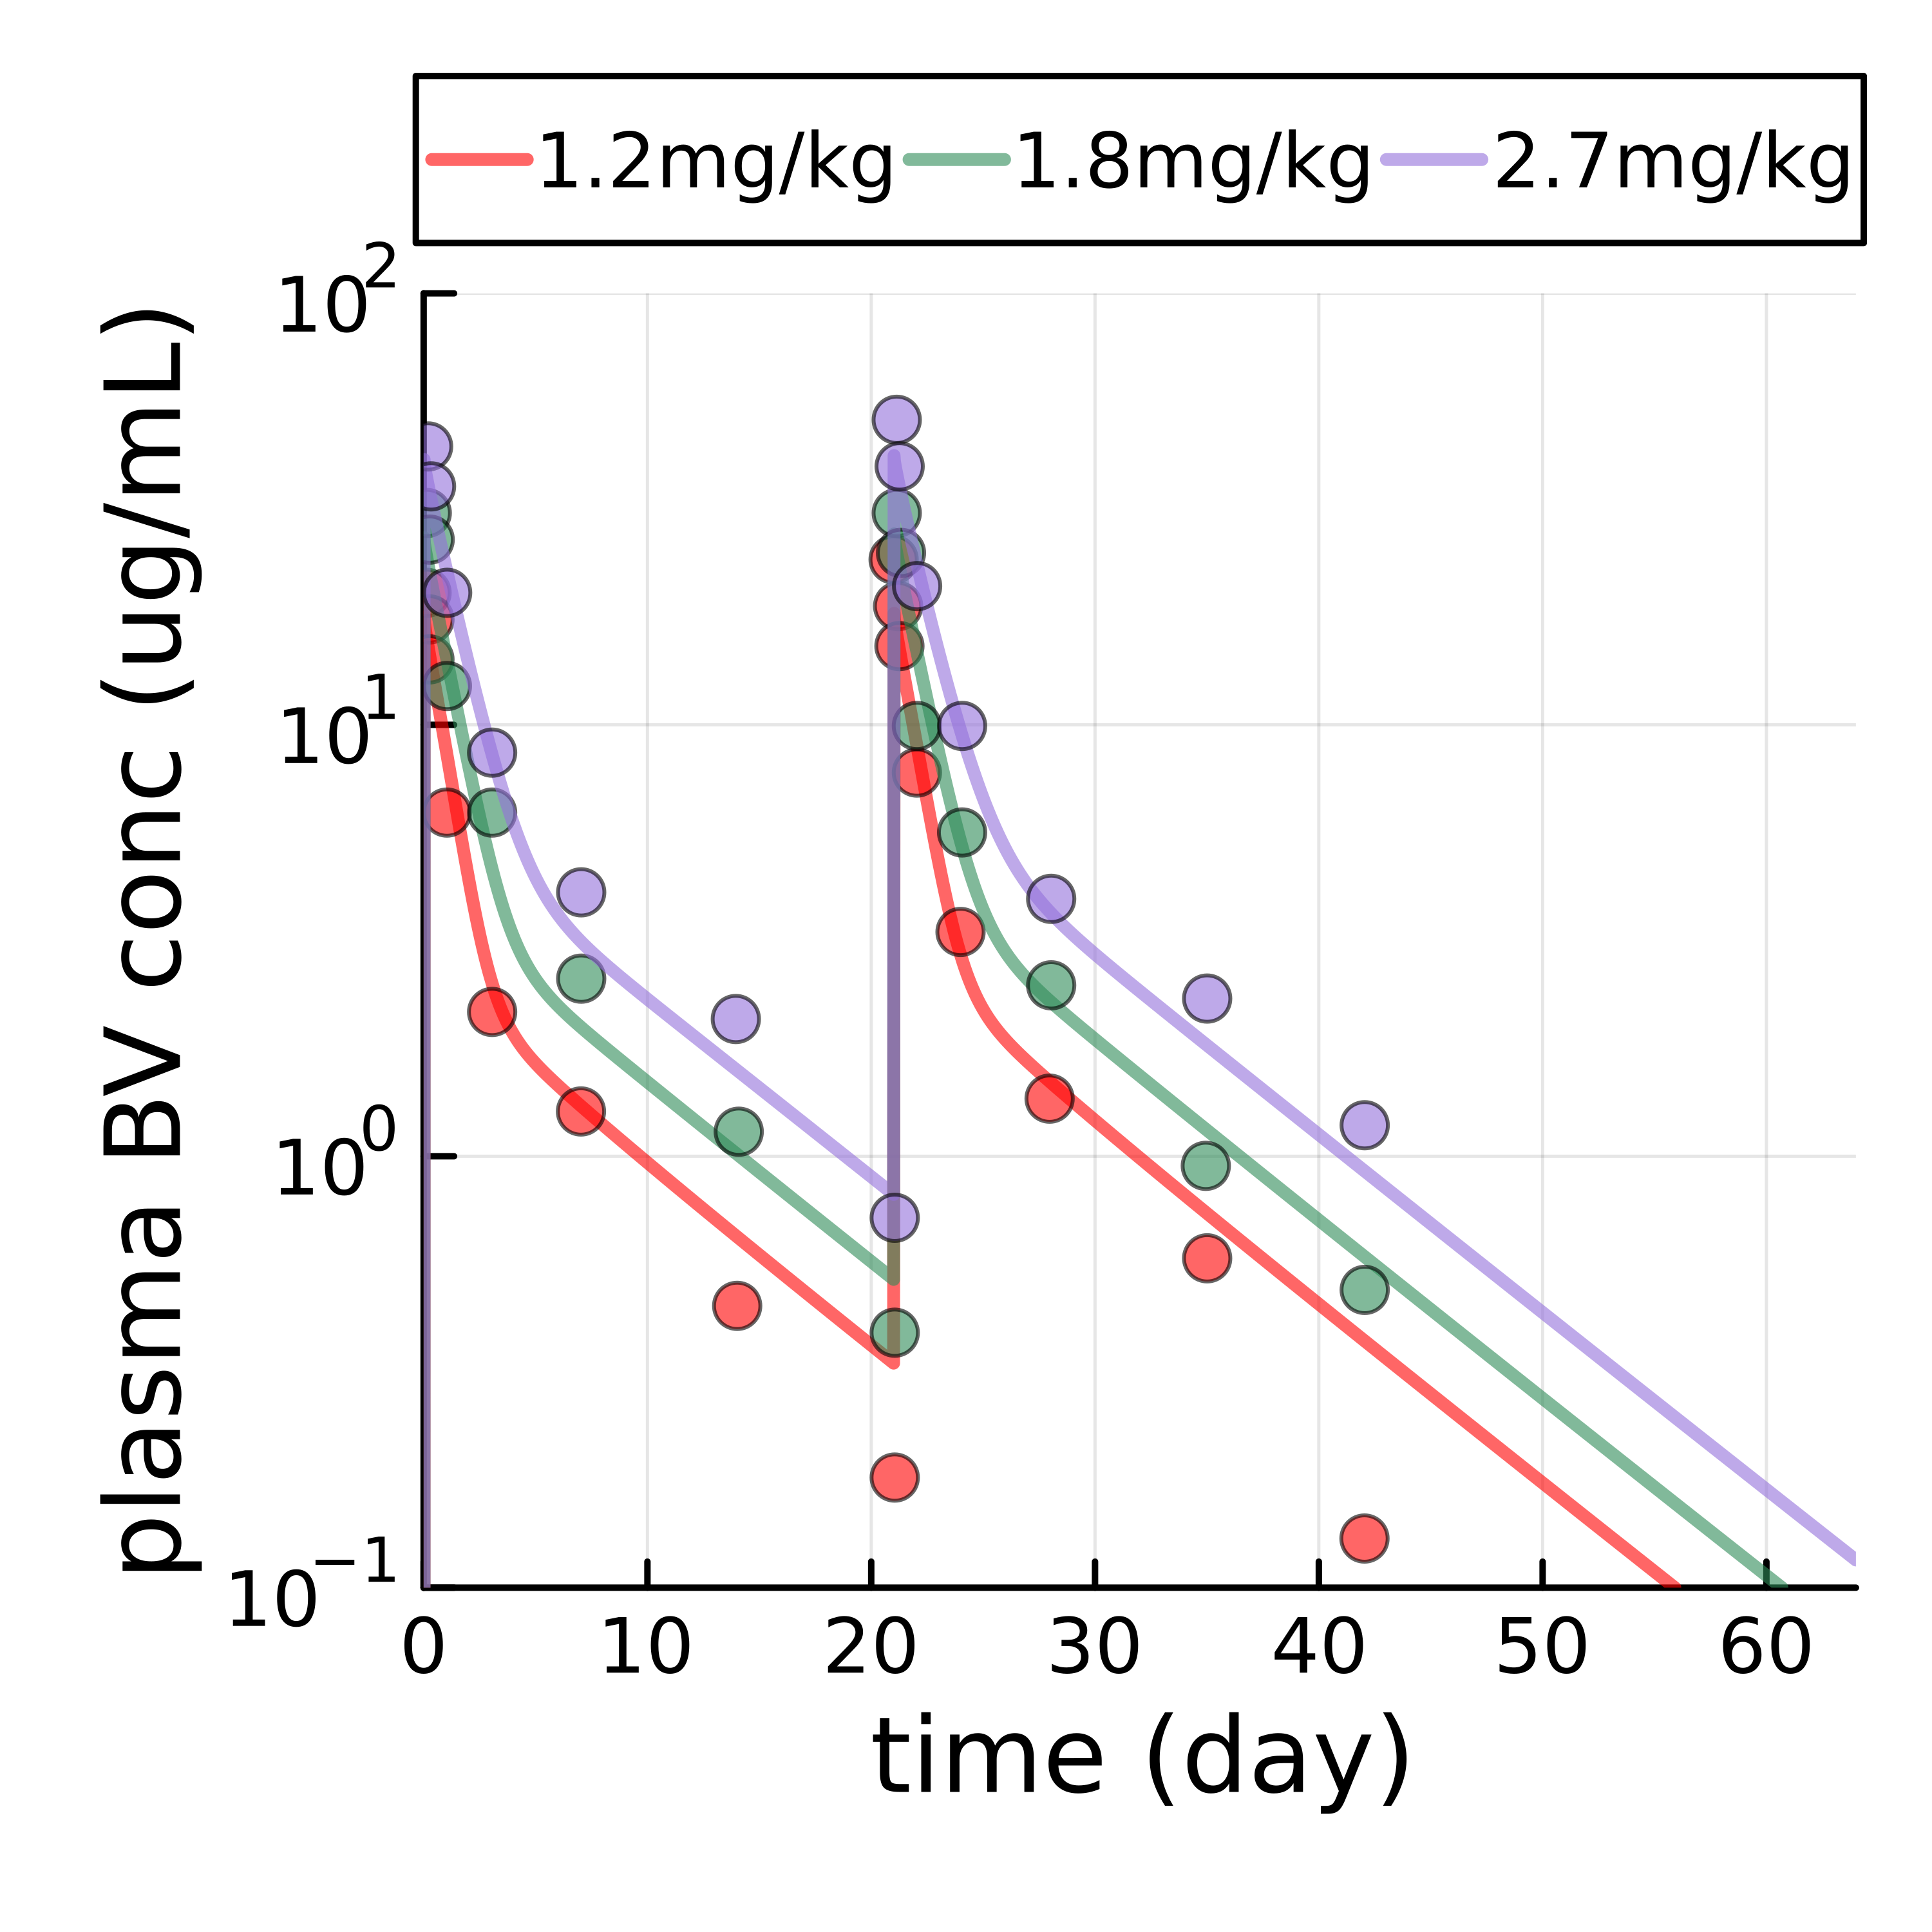
\includegraphics[width=\textwidth]{../img/brentuximab-vedotin-pk.png}
\scriptsize{Fig 2C. BV PK. (data source [6])}
\end{minipage}
\begin{minipage}[b]{0.24\linewidth}
\centering
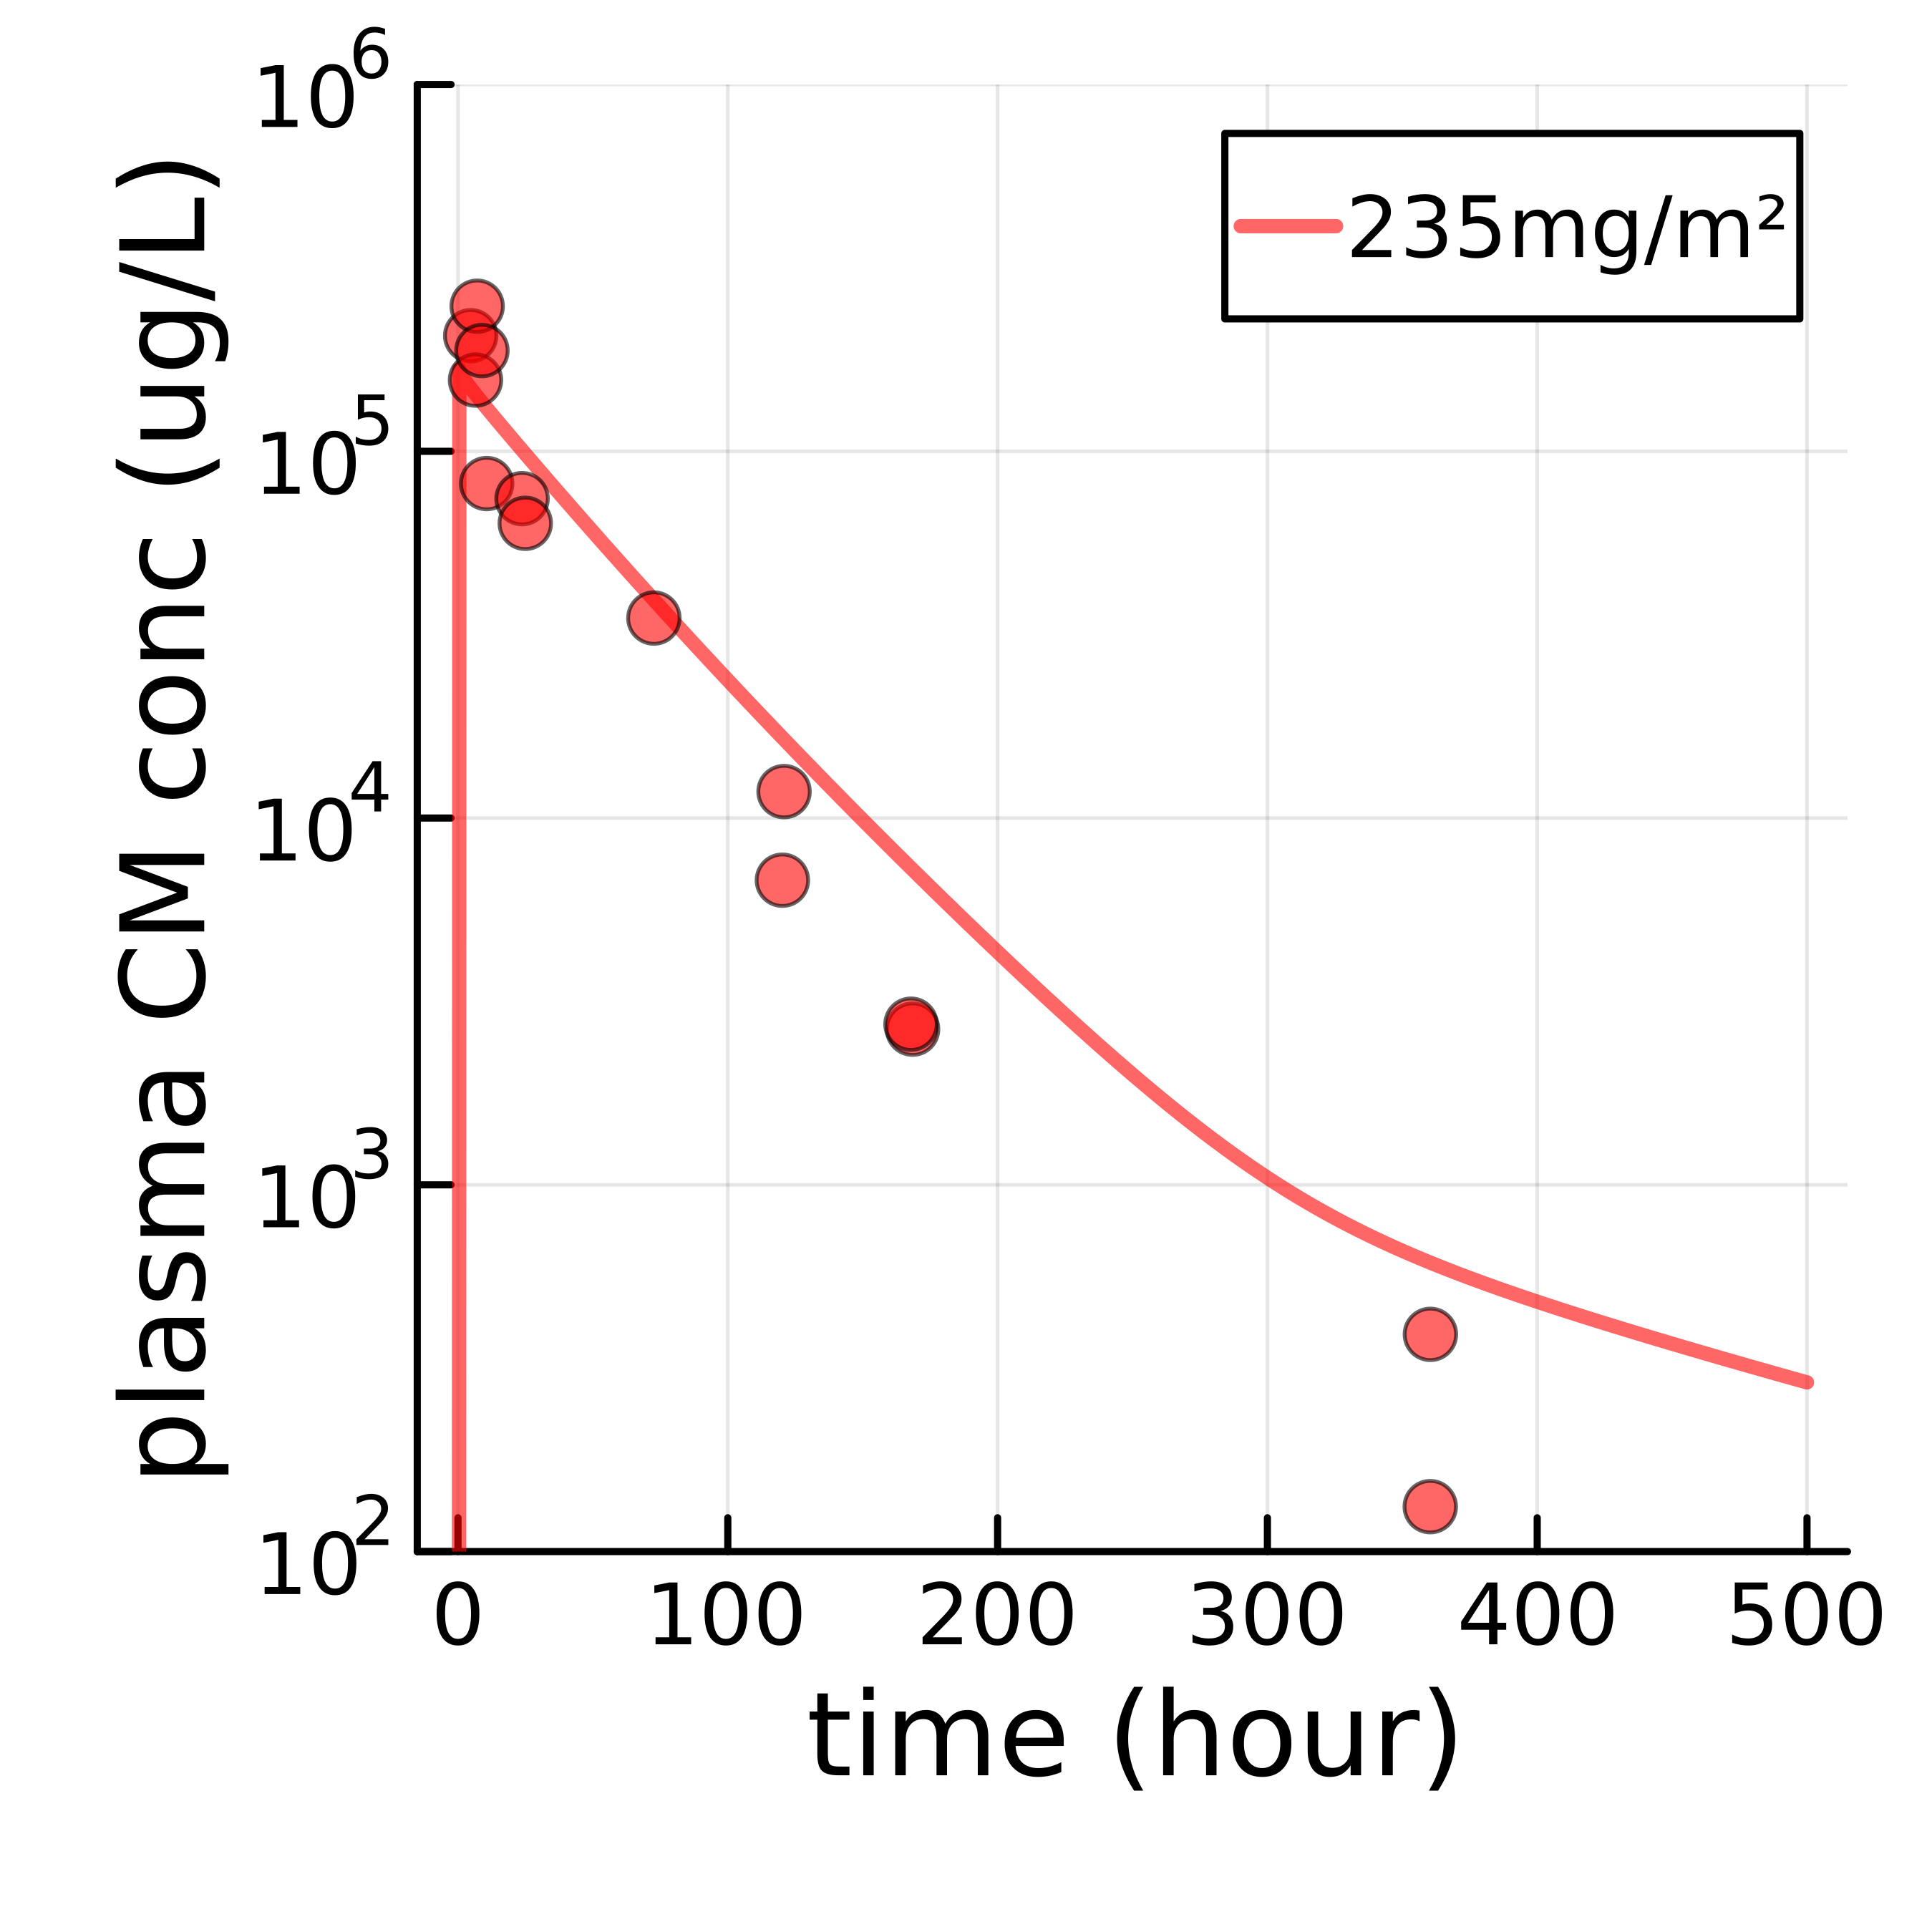
\includegraphics[width=\textwidth]{../img/cantuzumab-mertansine-pk.png}
\scriptsize{Fig 2D. CM PK. (data source [7])}
\end{minipage}

\smallskip

\begin{minipage}[ht]{0.42\linewidth}

The model predicted only \textbf{0.01\%} of the ADC dose reached the tumor, with the rest in organs such as liver (9.4\%), skin (3.7\%), and lung (3.6\%) (Fig 3A).
The ADC target receptor's internalization rate (Fig 3B) and receptor copy number (Fig 3C) were predicted to have limited impact on the amount of ADC destined for the tumor, indicating receptor expression was not the bottleneck.
The true predicted bottlenecks were the \textbf{tumor perfusion} (Fig. 3D) and the \textbf{ADC's diffusivity} (Fig. 3E), known limitations of ADCs in treating solid tumors [8].

\end{minipage}
\hspace{0.01\linewidth}
\begin{minipage}[ht]{0.3\linewidth}
\centering
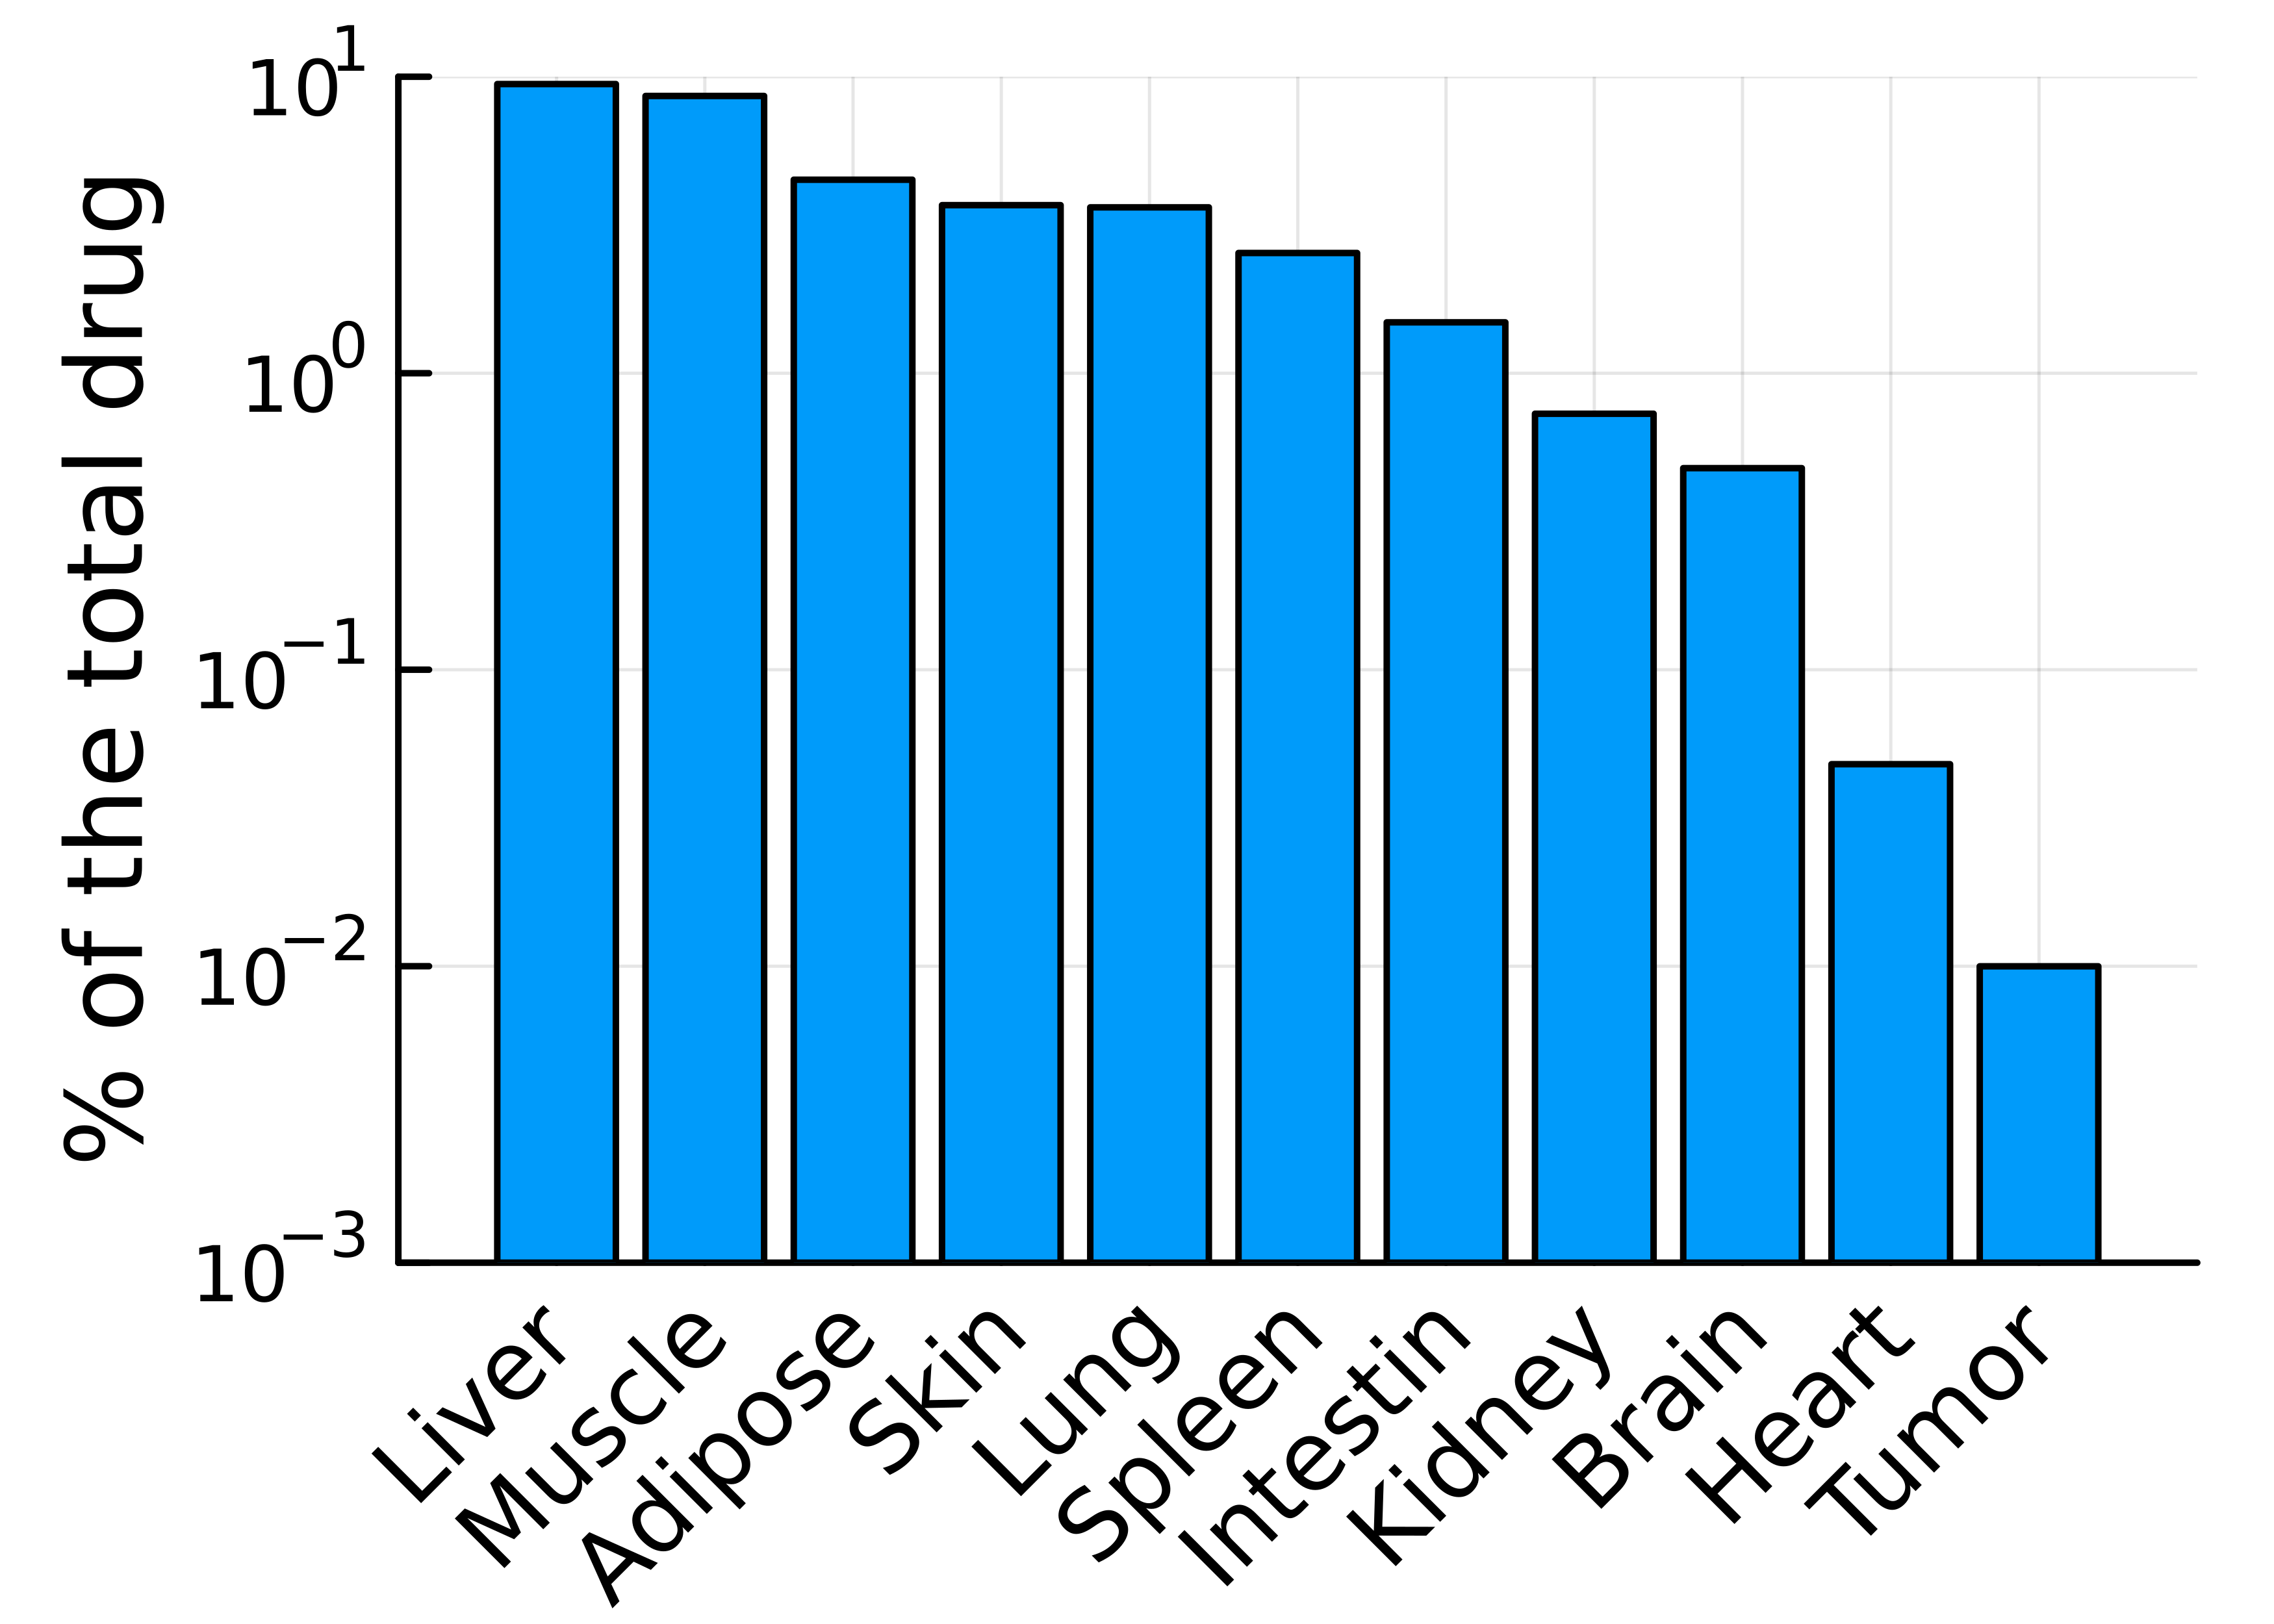
\includegraphics[width= \textwidth]{../img/t-dm1-total-mass-tissue.png}
\scriptsize{Fig 3A. Predicted T-DM1 in tissues }
\end{minipage}
\hspace{0.01\linewidth}
\begin{minipage}[ht]{0.23\linewidth}
\begin{center}
\fontsize{7pt}{7pt}\selectfont
\textbf{Table 1}. ADC used in this study. \\
\begin{tabular}{ c c c }
\hline
ADC & mAb & Payload \\ 
\hline
T-Dxd & Trastuzumab & Dxd  \\  
T-DM1 & Trastuzumab & DM1 \\
BV & Brentuximab & MMAE  \\  
CM & Cantuzumab & DM1 \\  
\hline
\end{tabular}
\end{center}
\end{minipage}


% \smallskip

\begin{minipage}[ht]{0.23\linewidth}
\centering
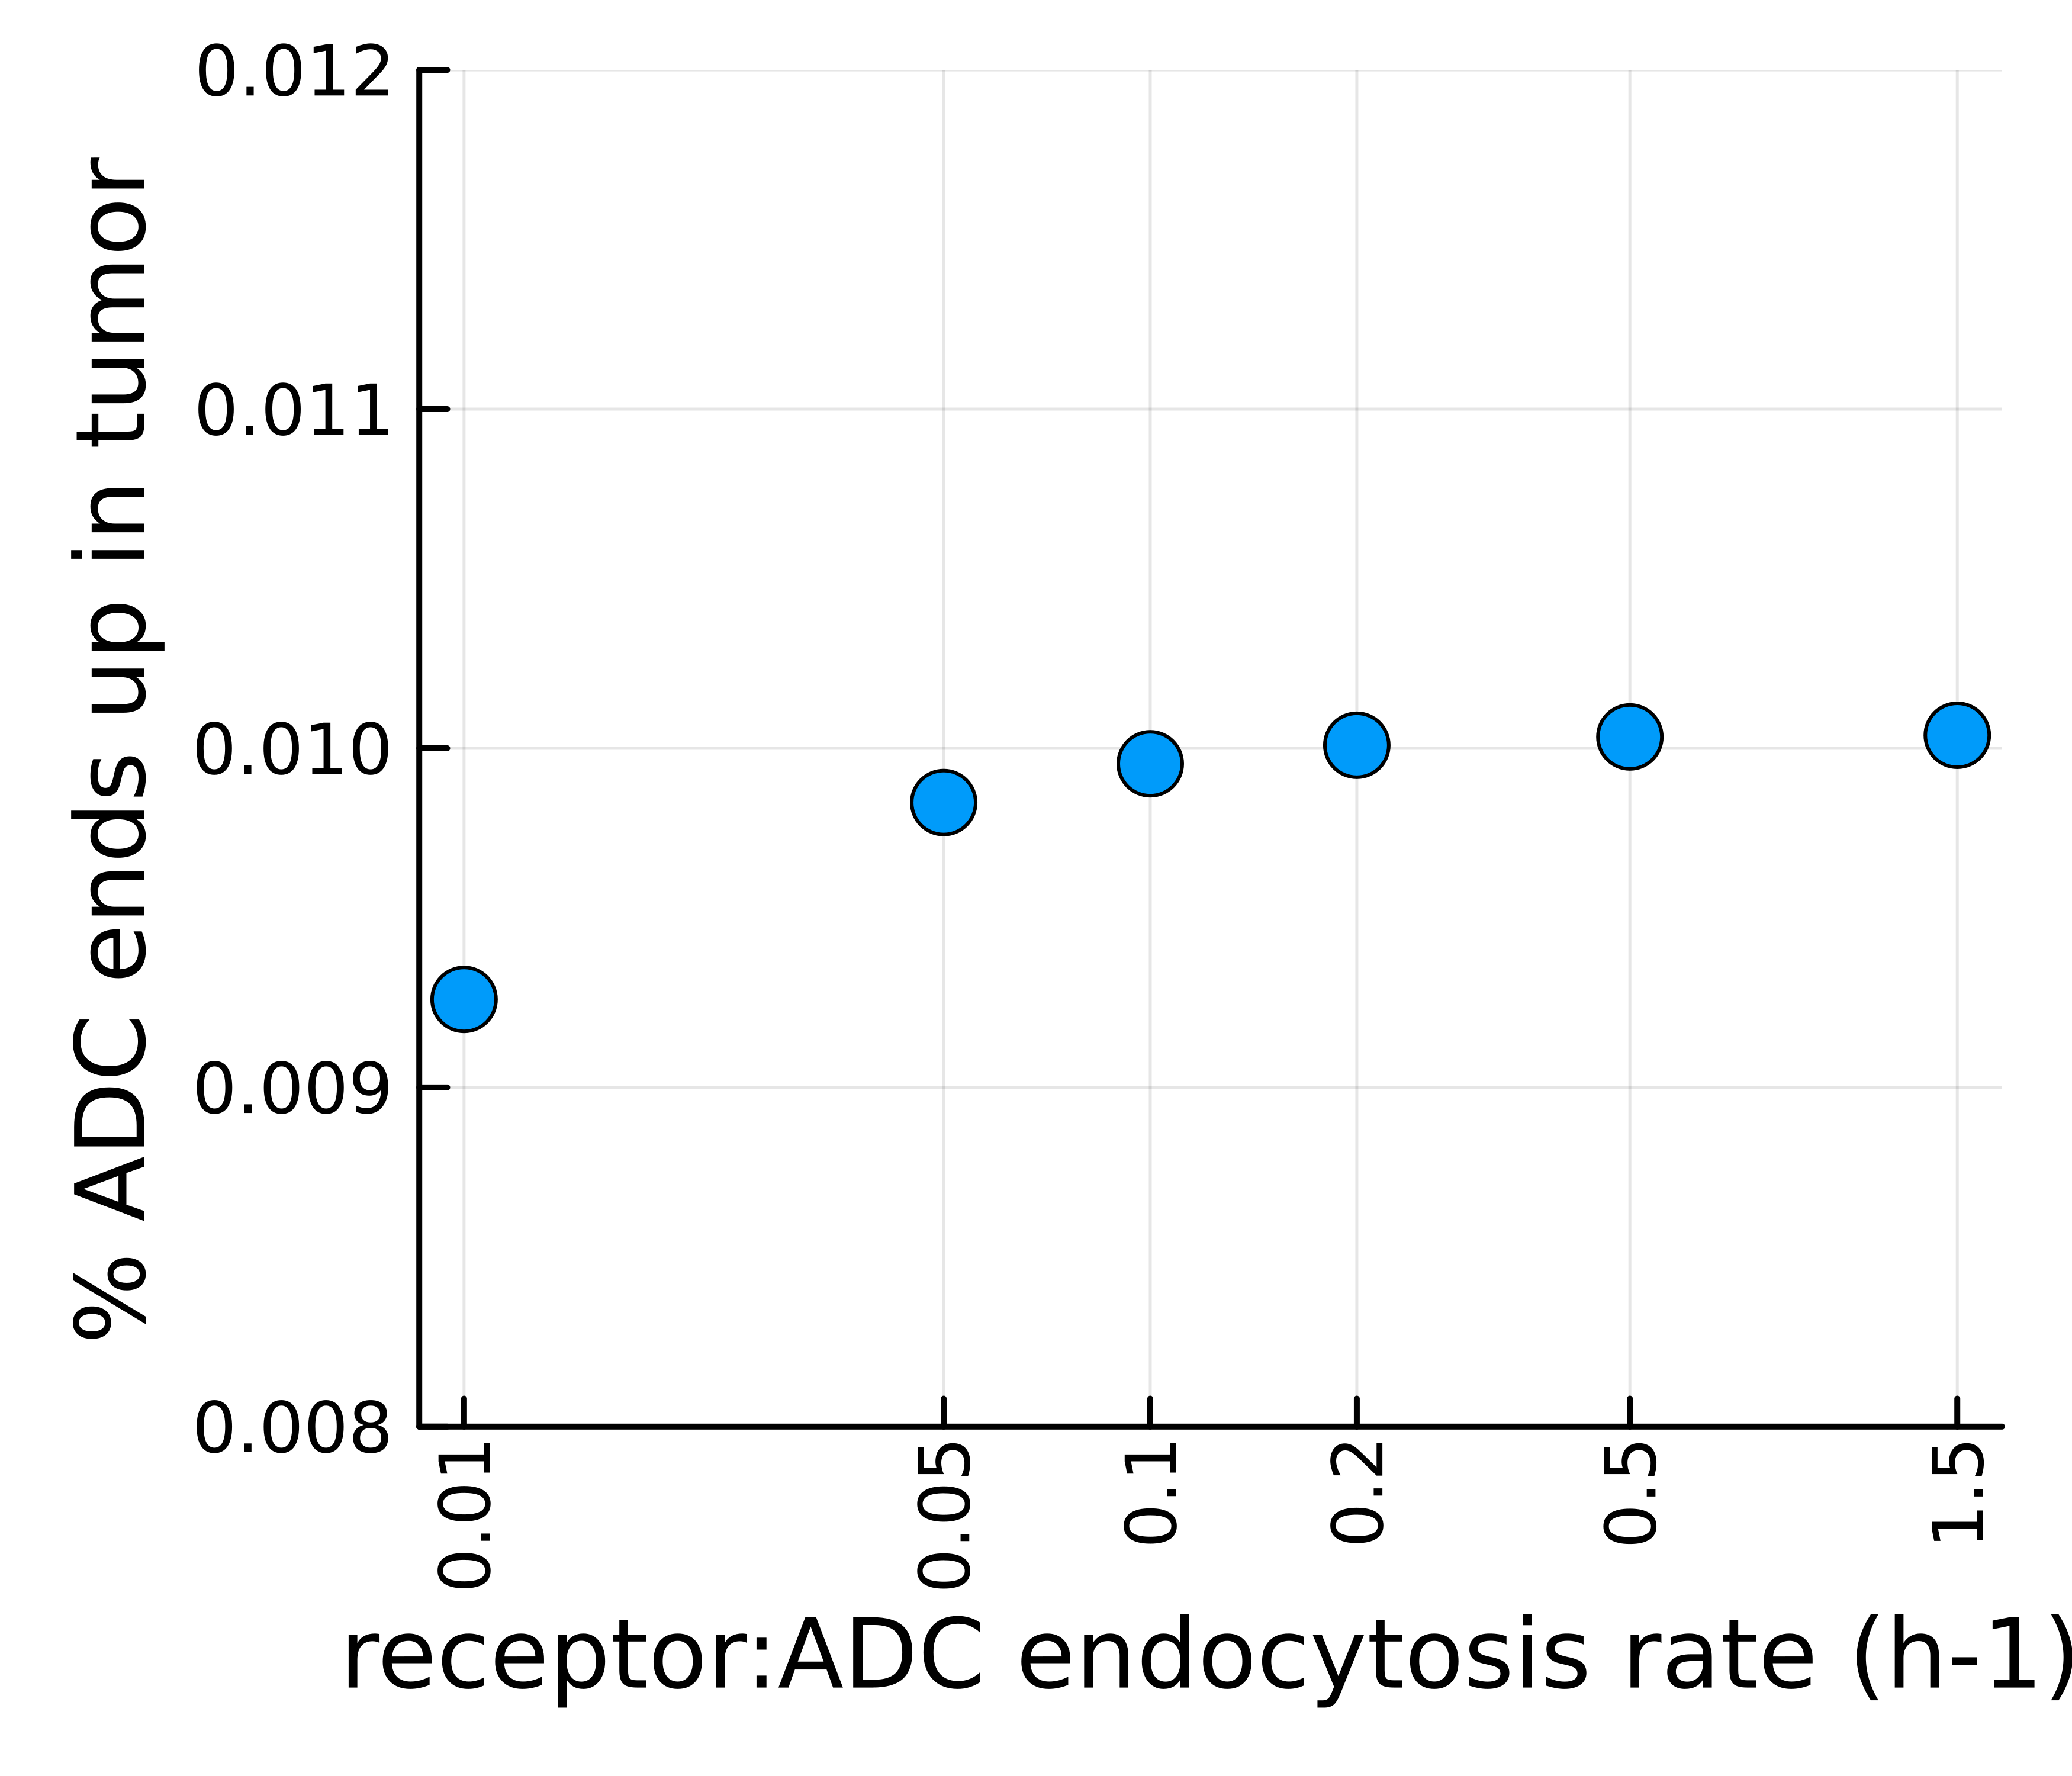
\includegraphics[width=\textwidth]{../img/param-scan/endocytosis-tumor-ADC-percentage.png}
\tiny{Fig 3B. Fraction of ADC dose predicted to reach the tumor vs. receptor:ADC internalization rates}
\end{minipage}
\hspace{0.2cm}
\begin{minipage}[ht]{0.23\linewidth}
\centering
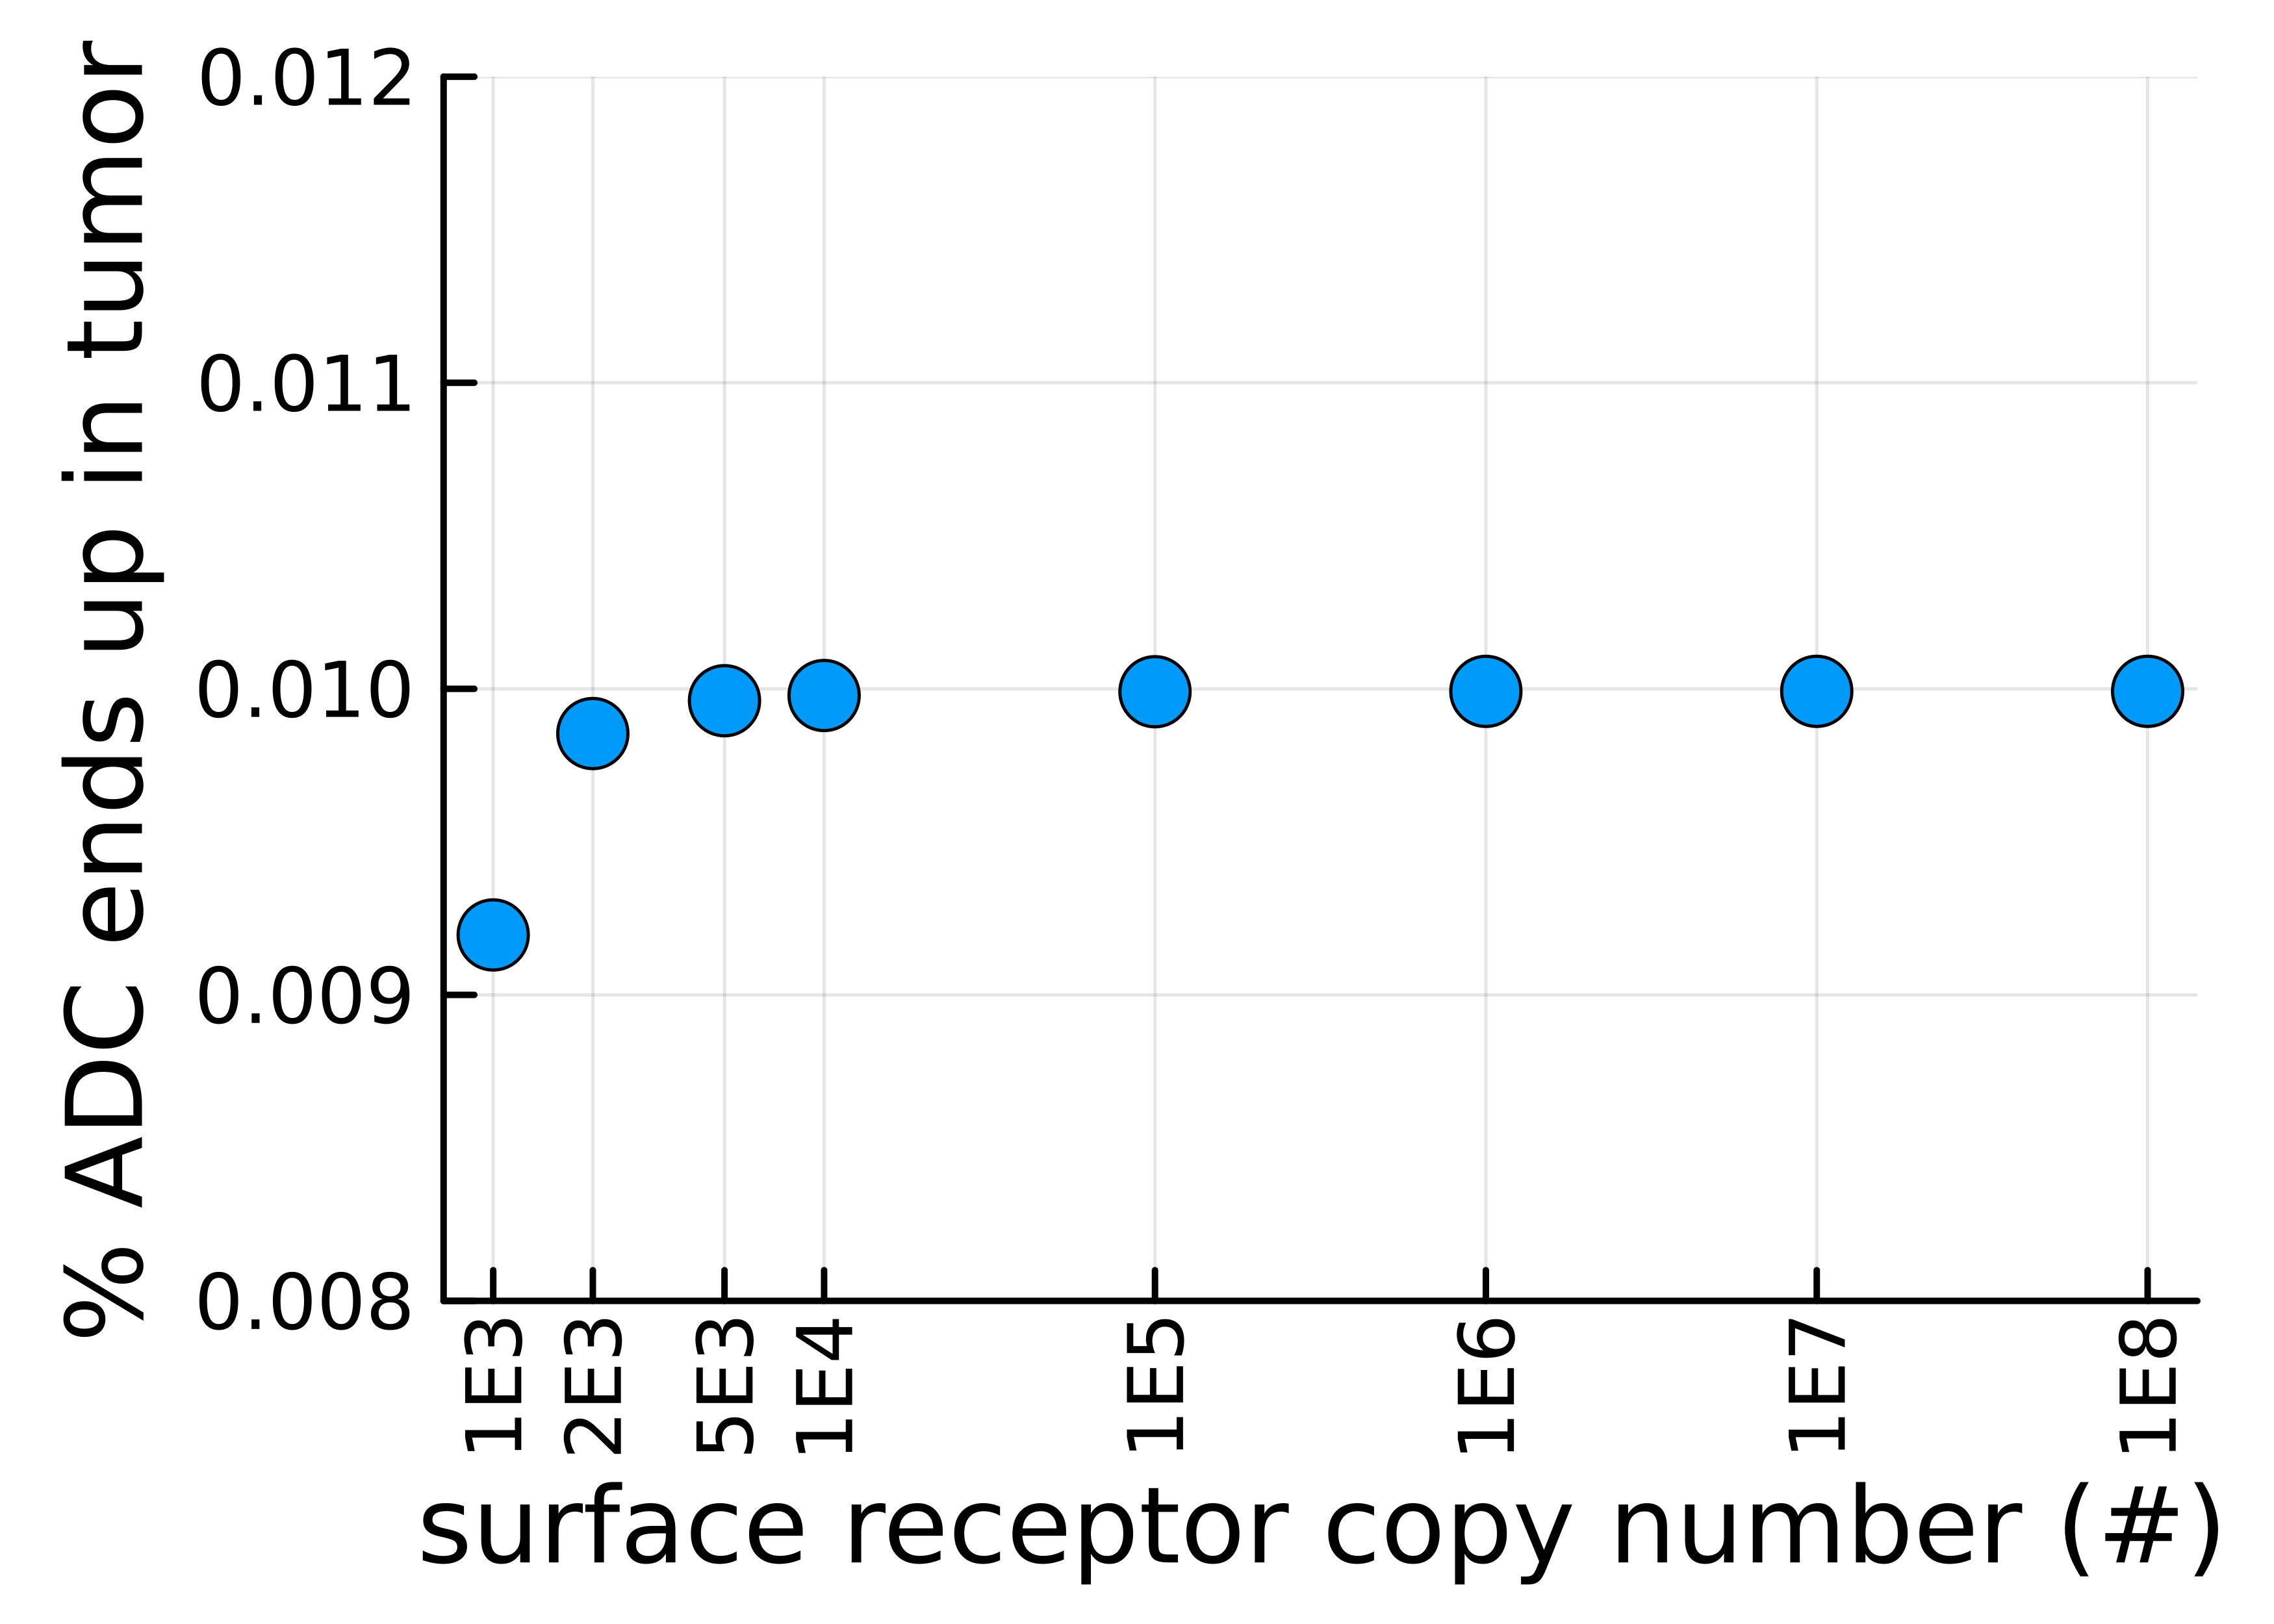
\includegraphics[width=\textwidth]{../img/param-scan/HER2-tumor-ADC-percentage.png}
\tiny{Fig 3C. Fraction of ADC dose predicted to reach the tumor  vs. receptor copy numbers per tumor cell}
\end{minipage}
\hspace{0.2cm}
\begin{minipage}[c]{0.23\linewidth}
\centering
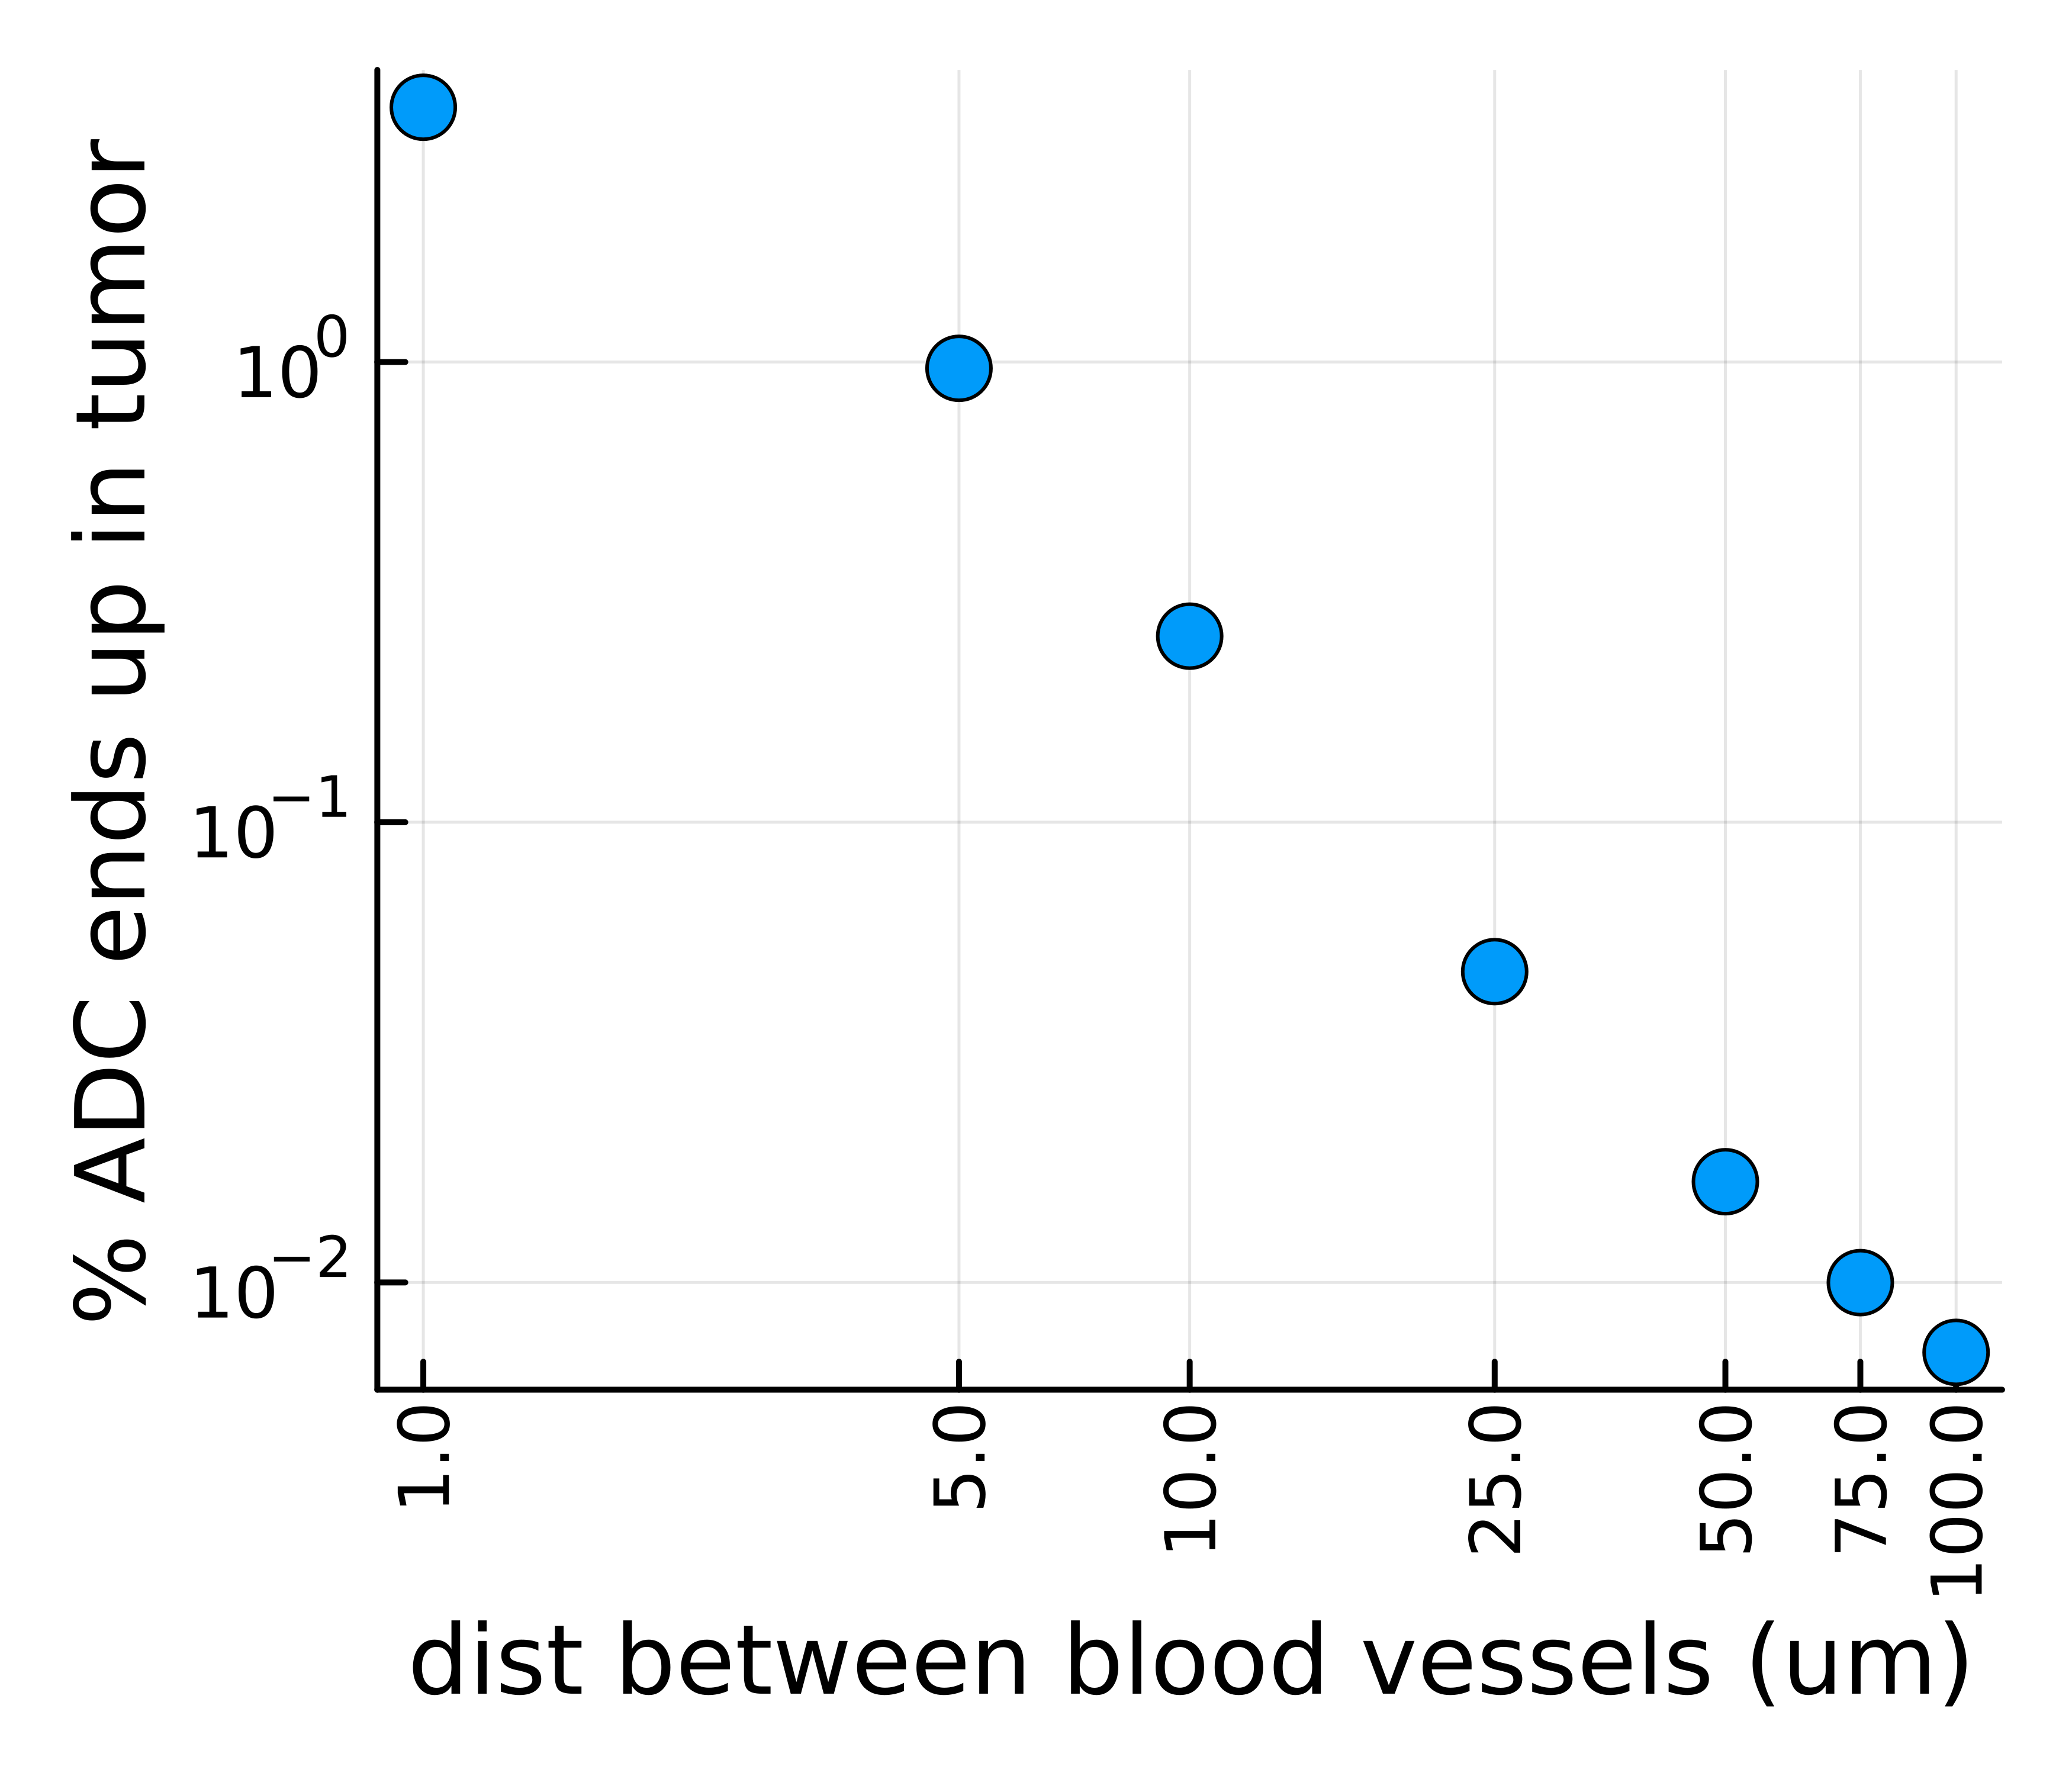
\includegraphics[width=\textwidth]{../img/param-scan/Rkrogh-tumor-ADC-percentage.png}
\tiny{Fig 3D. Fraction of ADC dose predicted to reach the tumor vs. tumor perfusion}
\end{minipage}
\hspace{0.2cm}
\begin{minipage}[c]{0.23\linewidth}
\centering
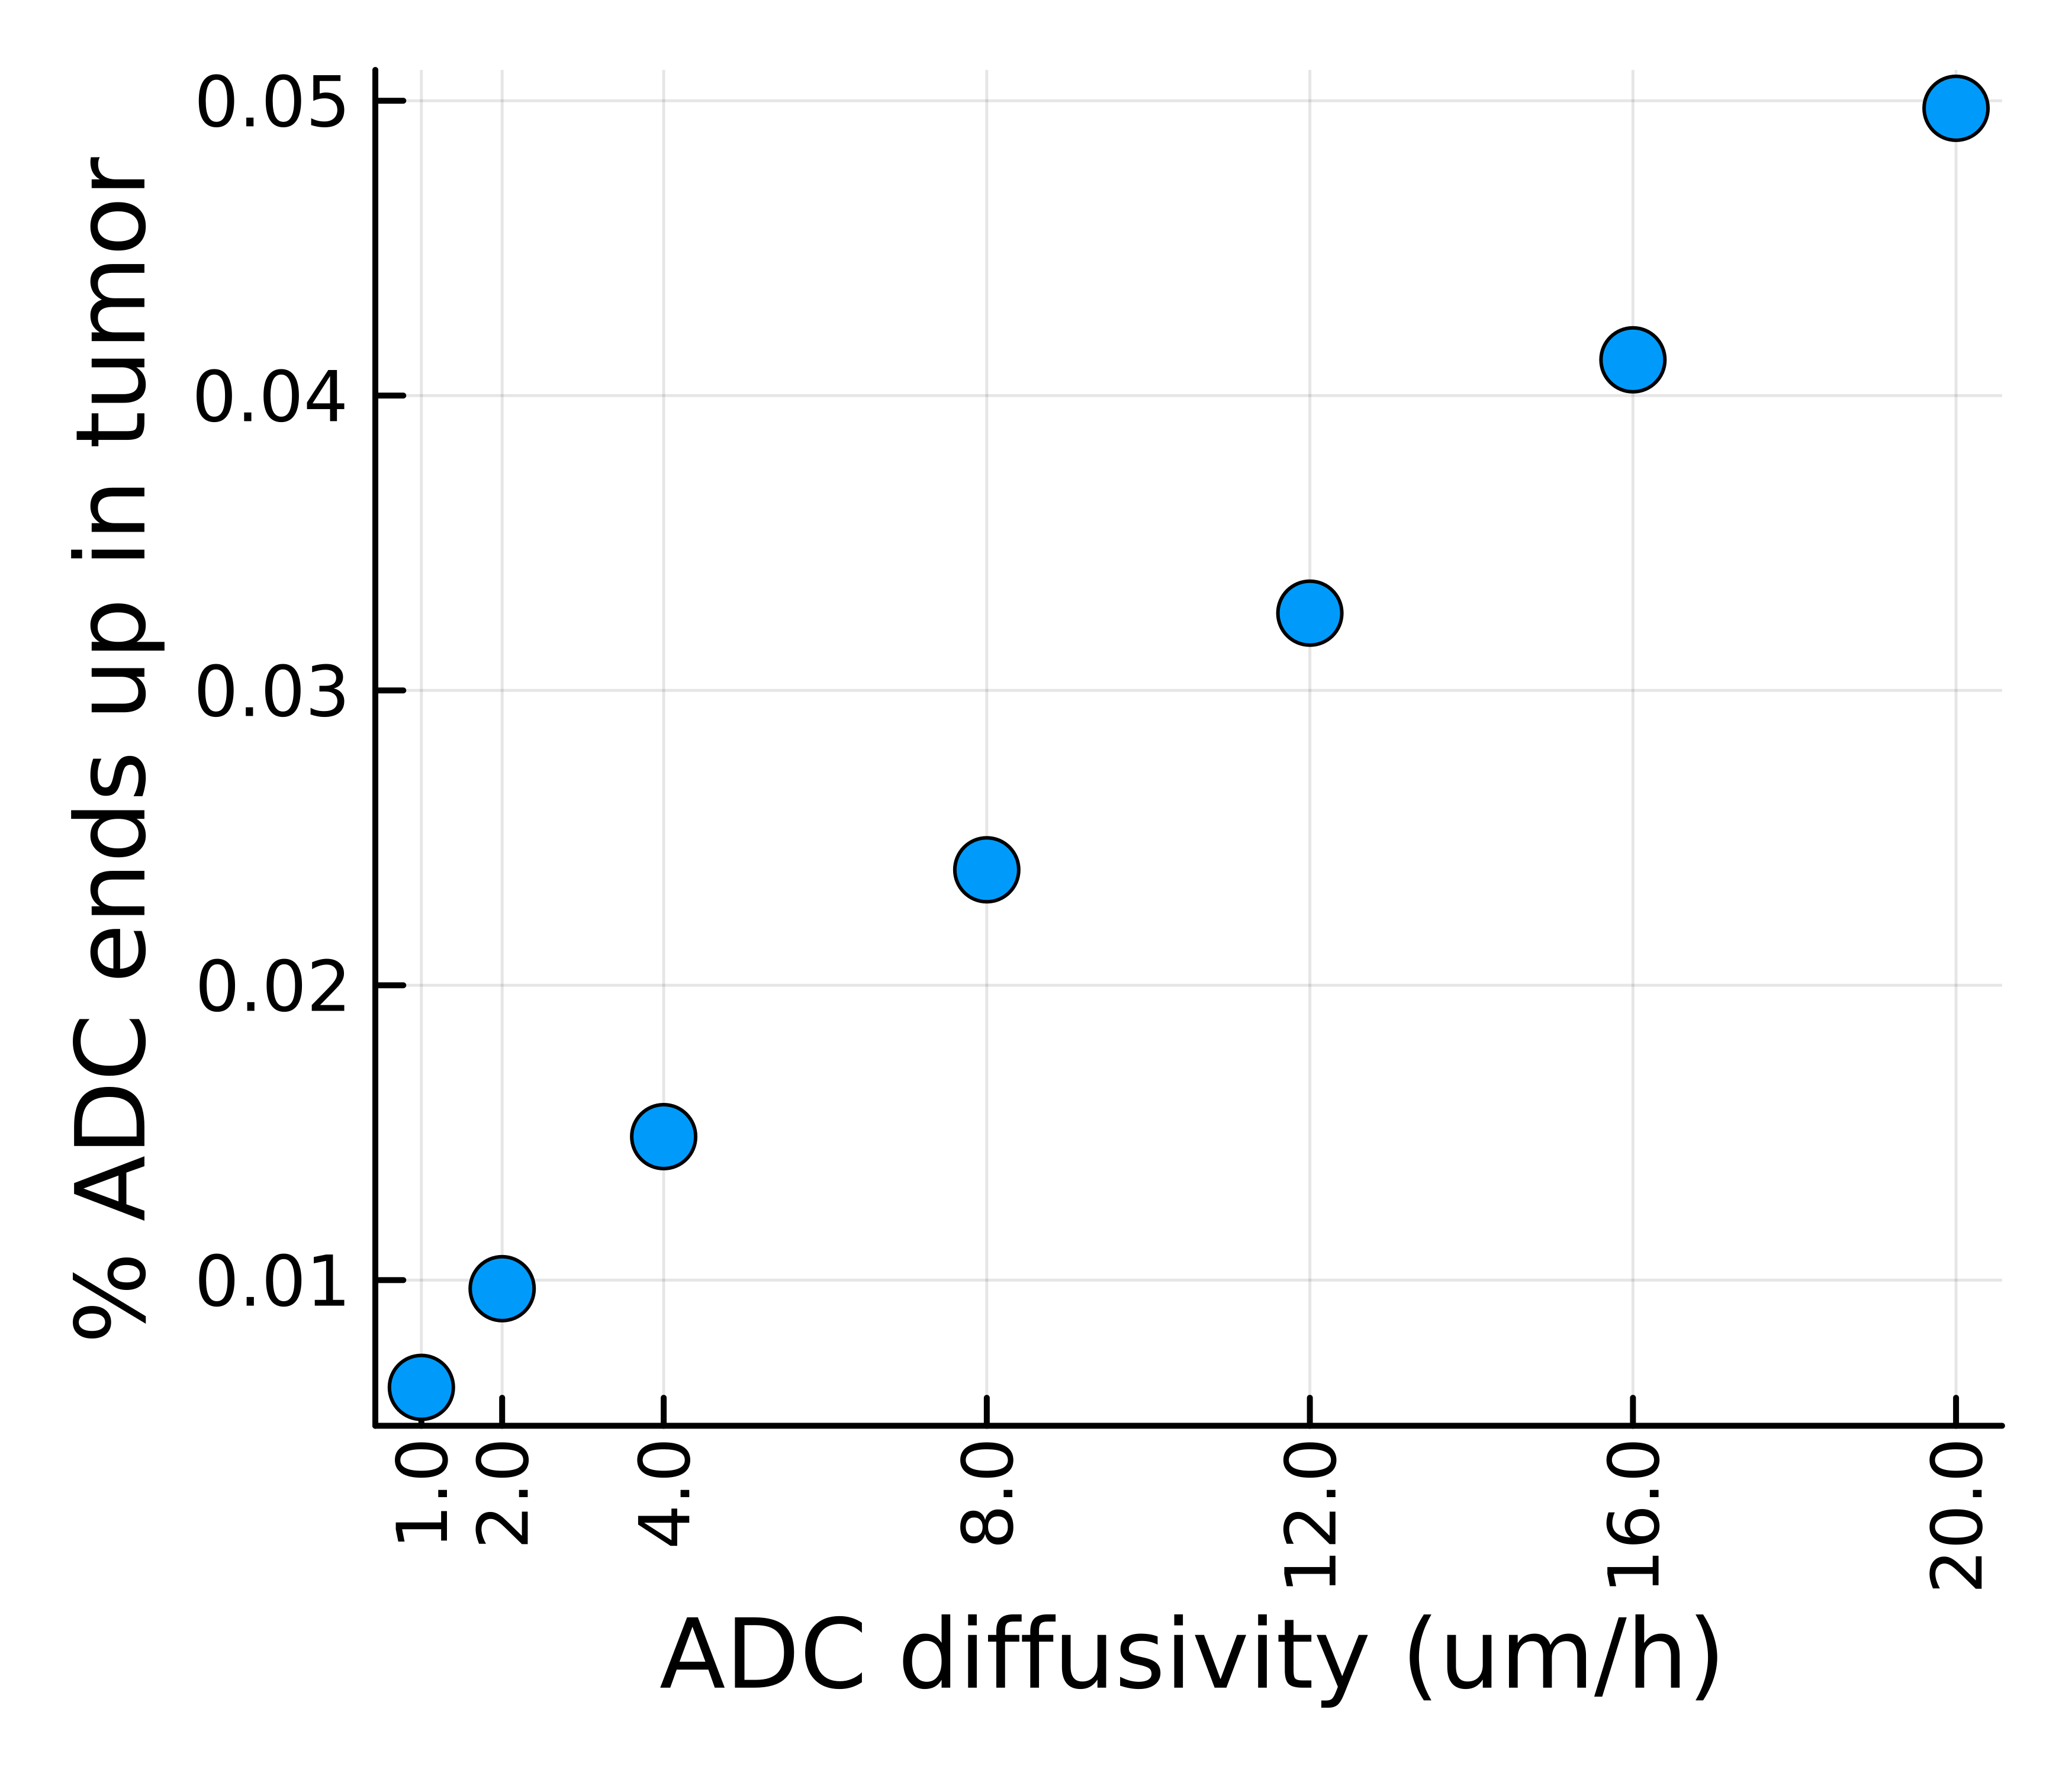
\includegraphics[width=\textwidth]{../img/param-scan/P-ADC-tumor-ADC-percentage.png}
\tiny{Fig 3E. Fraction of ADC dose predicted to reach the tumor vs. ADC diffusion rate}
\end{minipage}

\medskip


\begin{minipage}[c]{0.62\linewidth}

The \textbf{systemic distribution of ADC in interstitial fluids} should be considered a source of potential \textbf{\color{metgreen}{on-target off-tumor toxicity}}. 
The model predicted ADC concentrations >IC50 in lung,  skin, and small intestine interstitia (Fig 4). 
Given the presence of HER2+ cells in these organs, ADC in tissue interstitium may explain toxicities observed in T-DM1 [9]. 

\end{minipage}
\hspace{0.1cm}
\begin{minipage}[c]{0.32\linewidth}
\centering
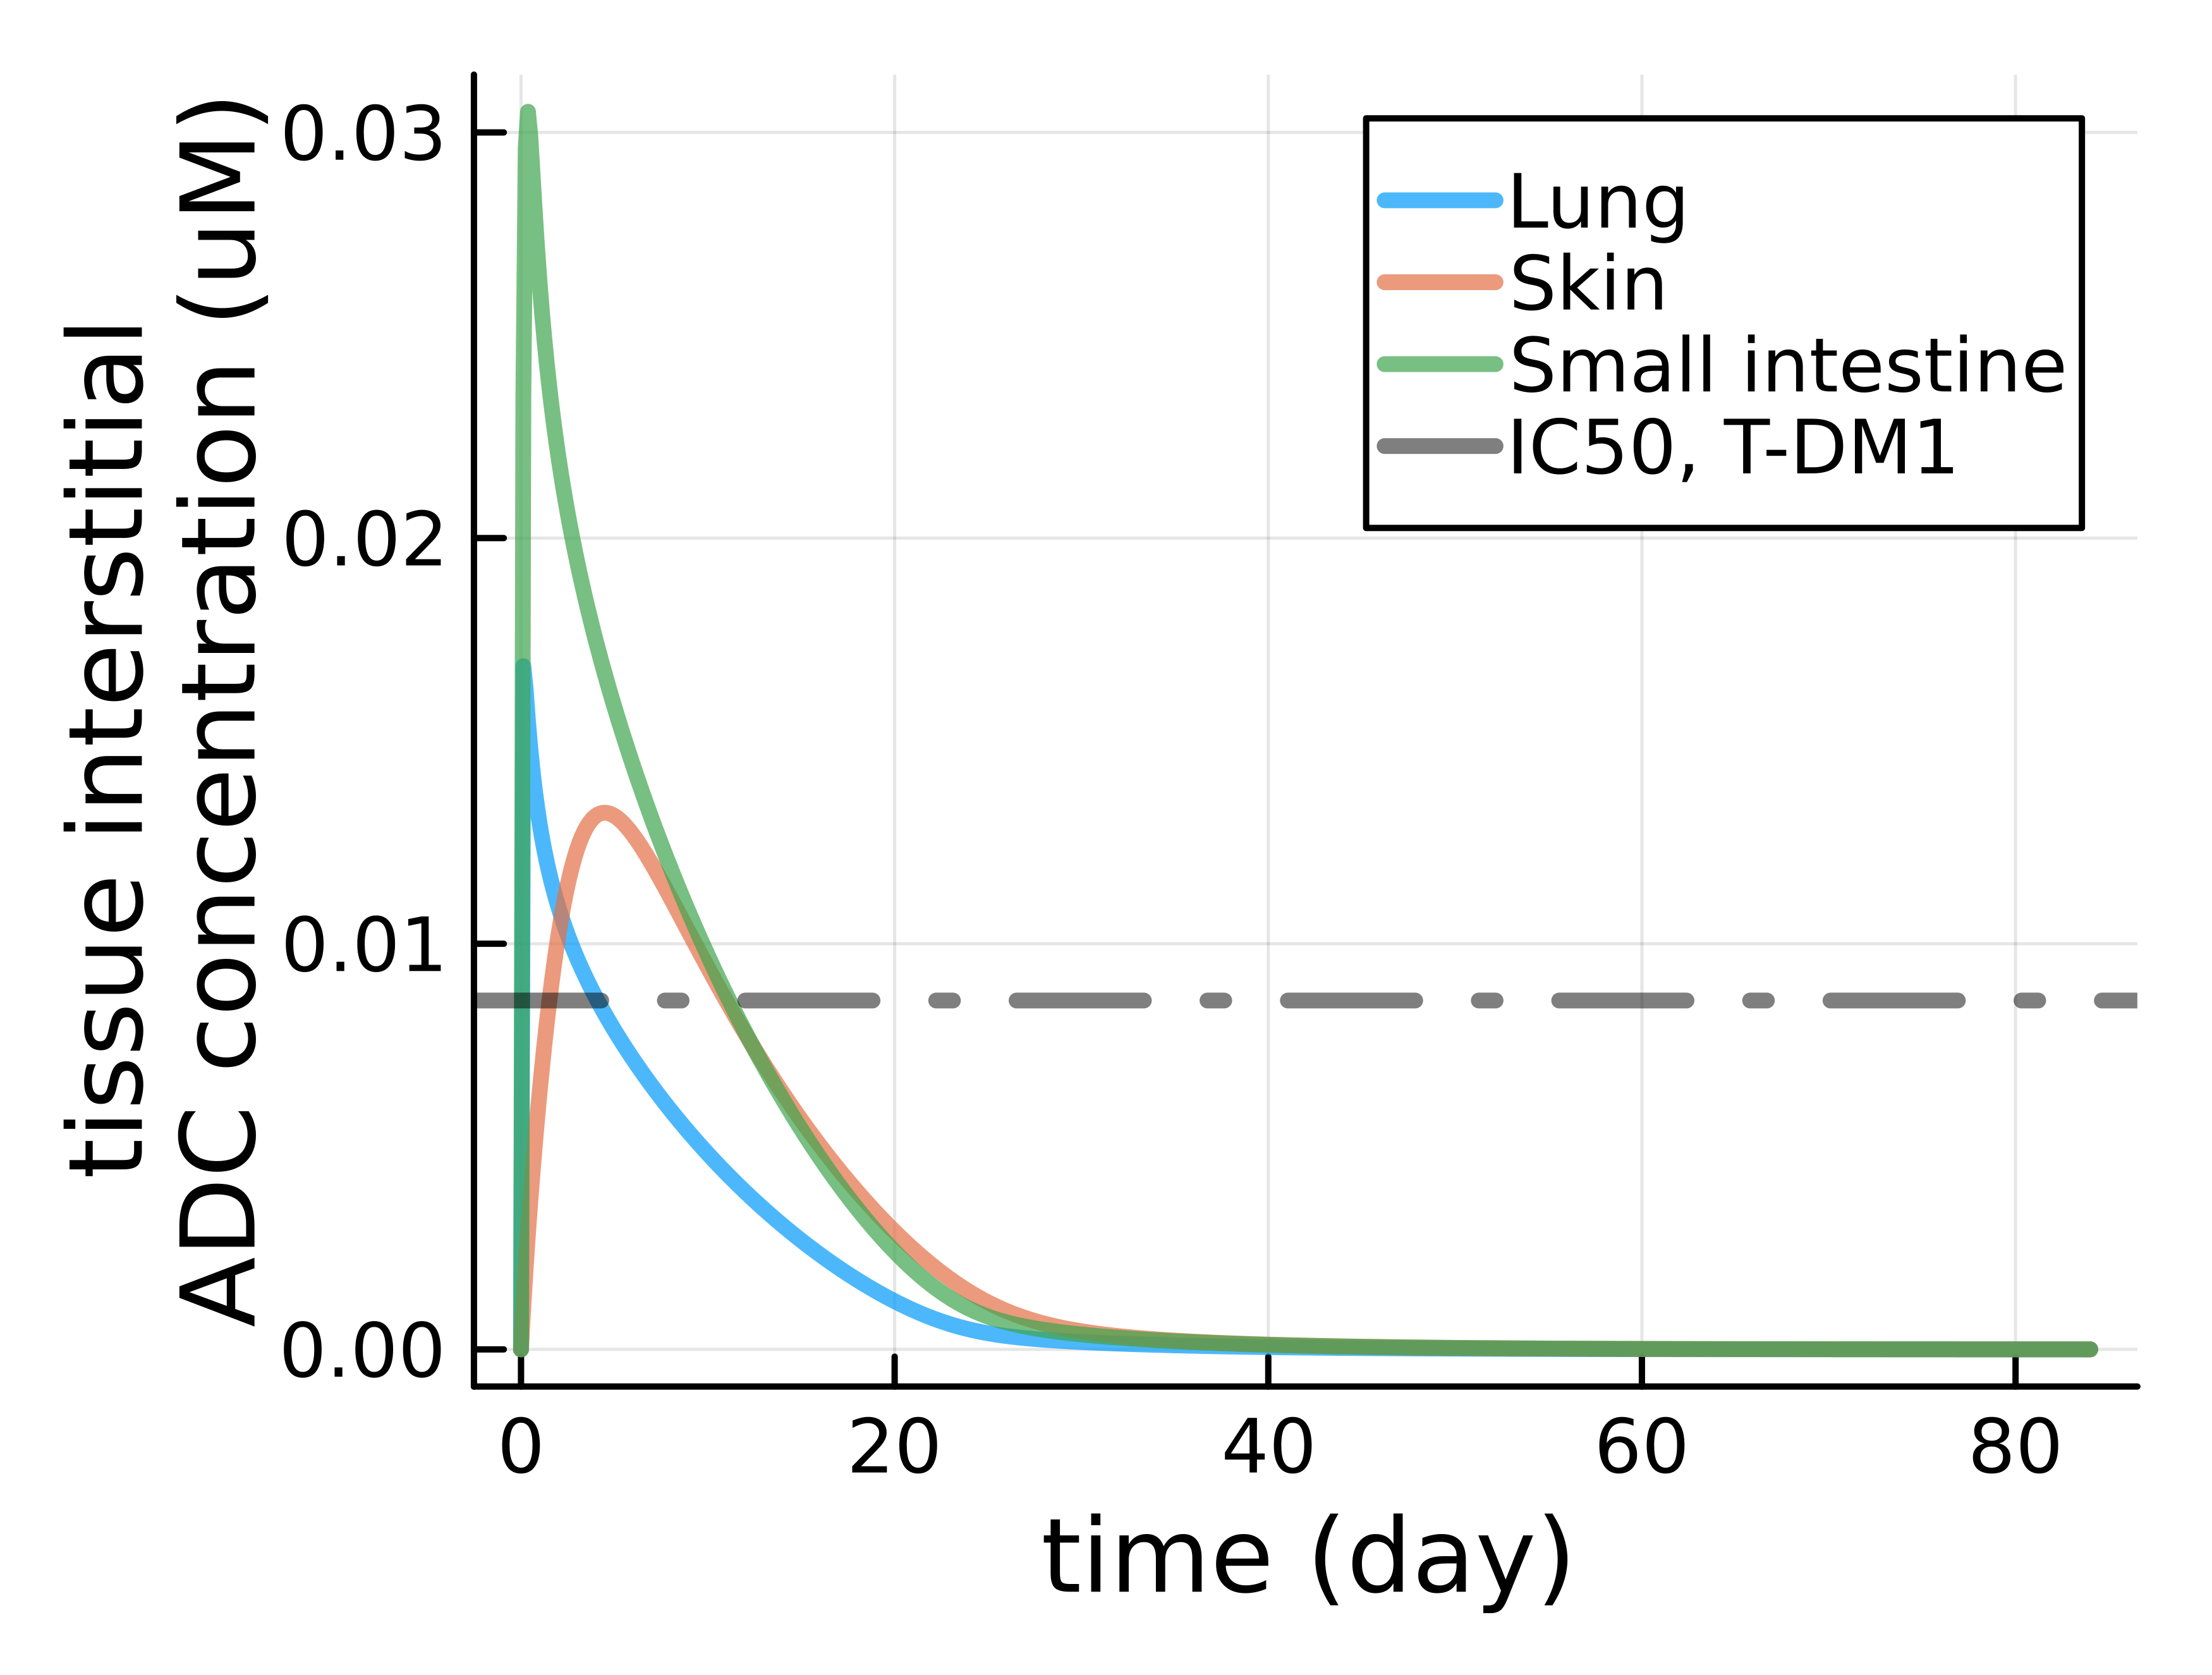
\includegraphics[width= 0.8 \textwidth]{../img/t-dm1-tissue-ints.png} \\
\scriptsize{Fig 4. Predicted interstitial T-DM1 conc}
\end{minipage}

\smallskip

\textbf{Free payload} could be a source of \textbf{\color{metgreen}{off-target toxicity}}. 
Predicted DM1 concentration >IC50 in liver endothelial cells after a dose of 3.6mg/kg T-DM1, consistent with the hepatic toxicity observed in T-DM1 (Fig 5A). 
Predicted Dxd and MMAE concentrations were lower than their IC50 after a dose of 5.4mg/kg T-Dxd and 1.2mg/kg BV (Fig 5B, C), respectively, consistent with the lack of hepatic toxicity observed in T-Dxd and BV [10].

\begin{minipage}[c]{0.33\linewidth}
\centering
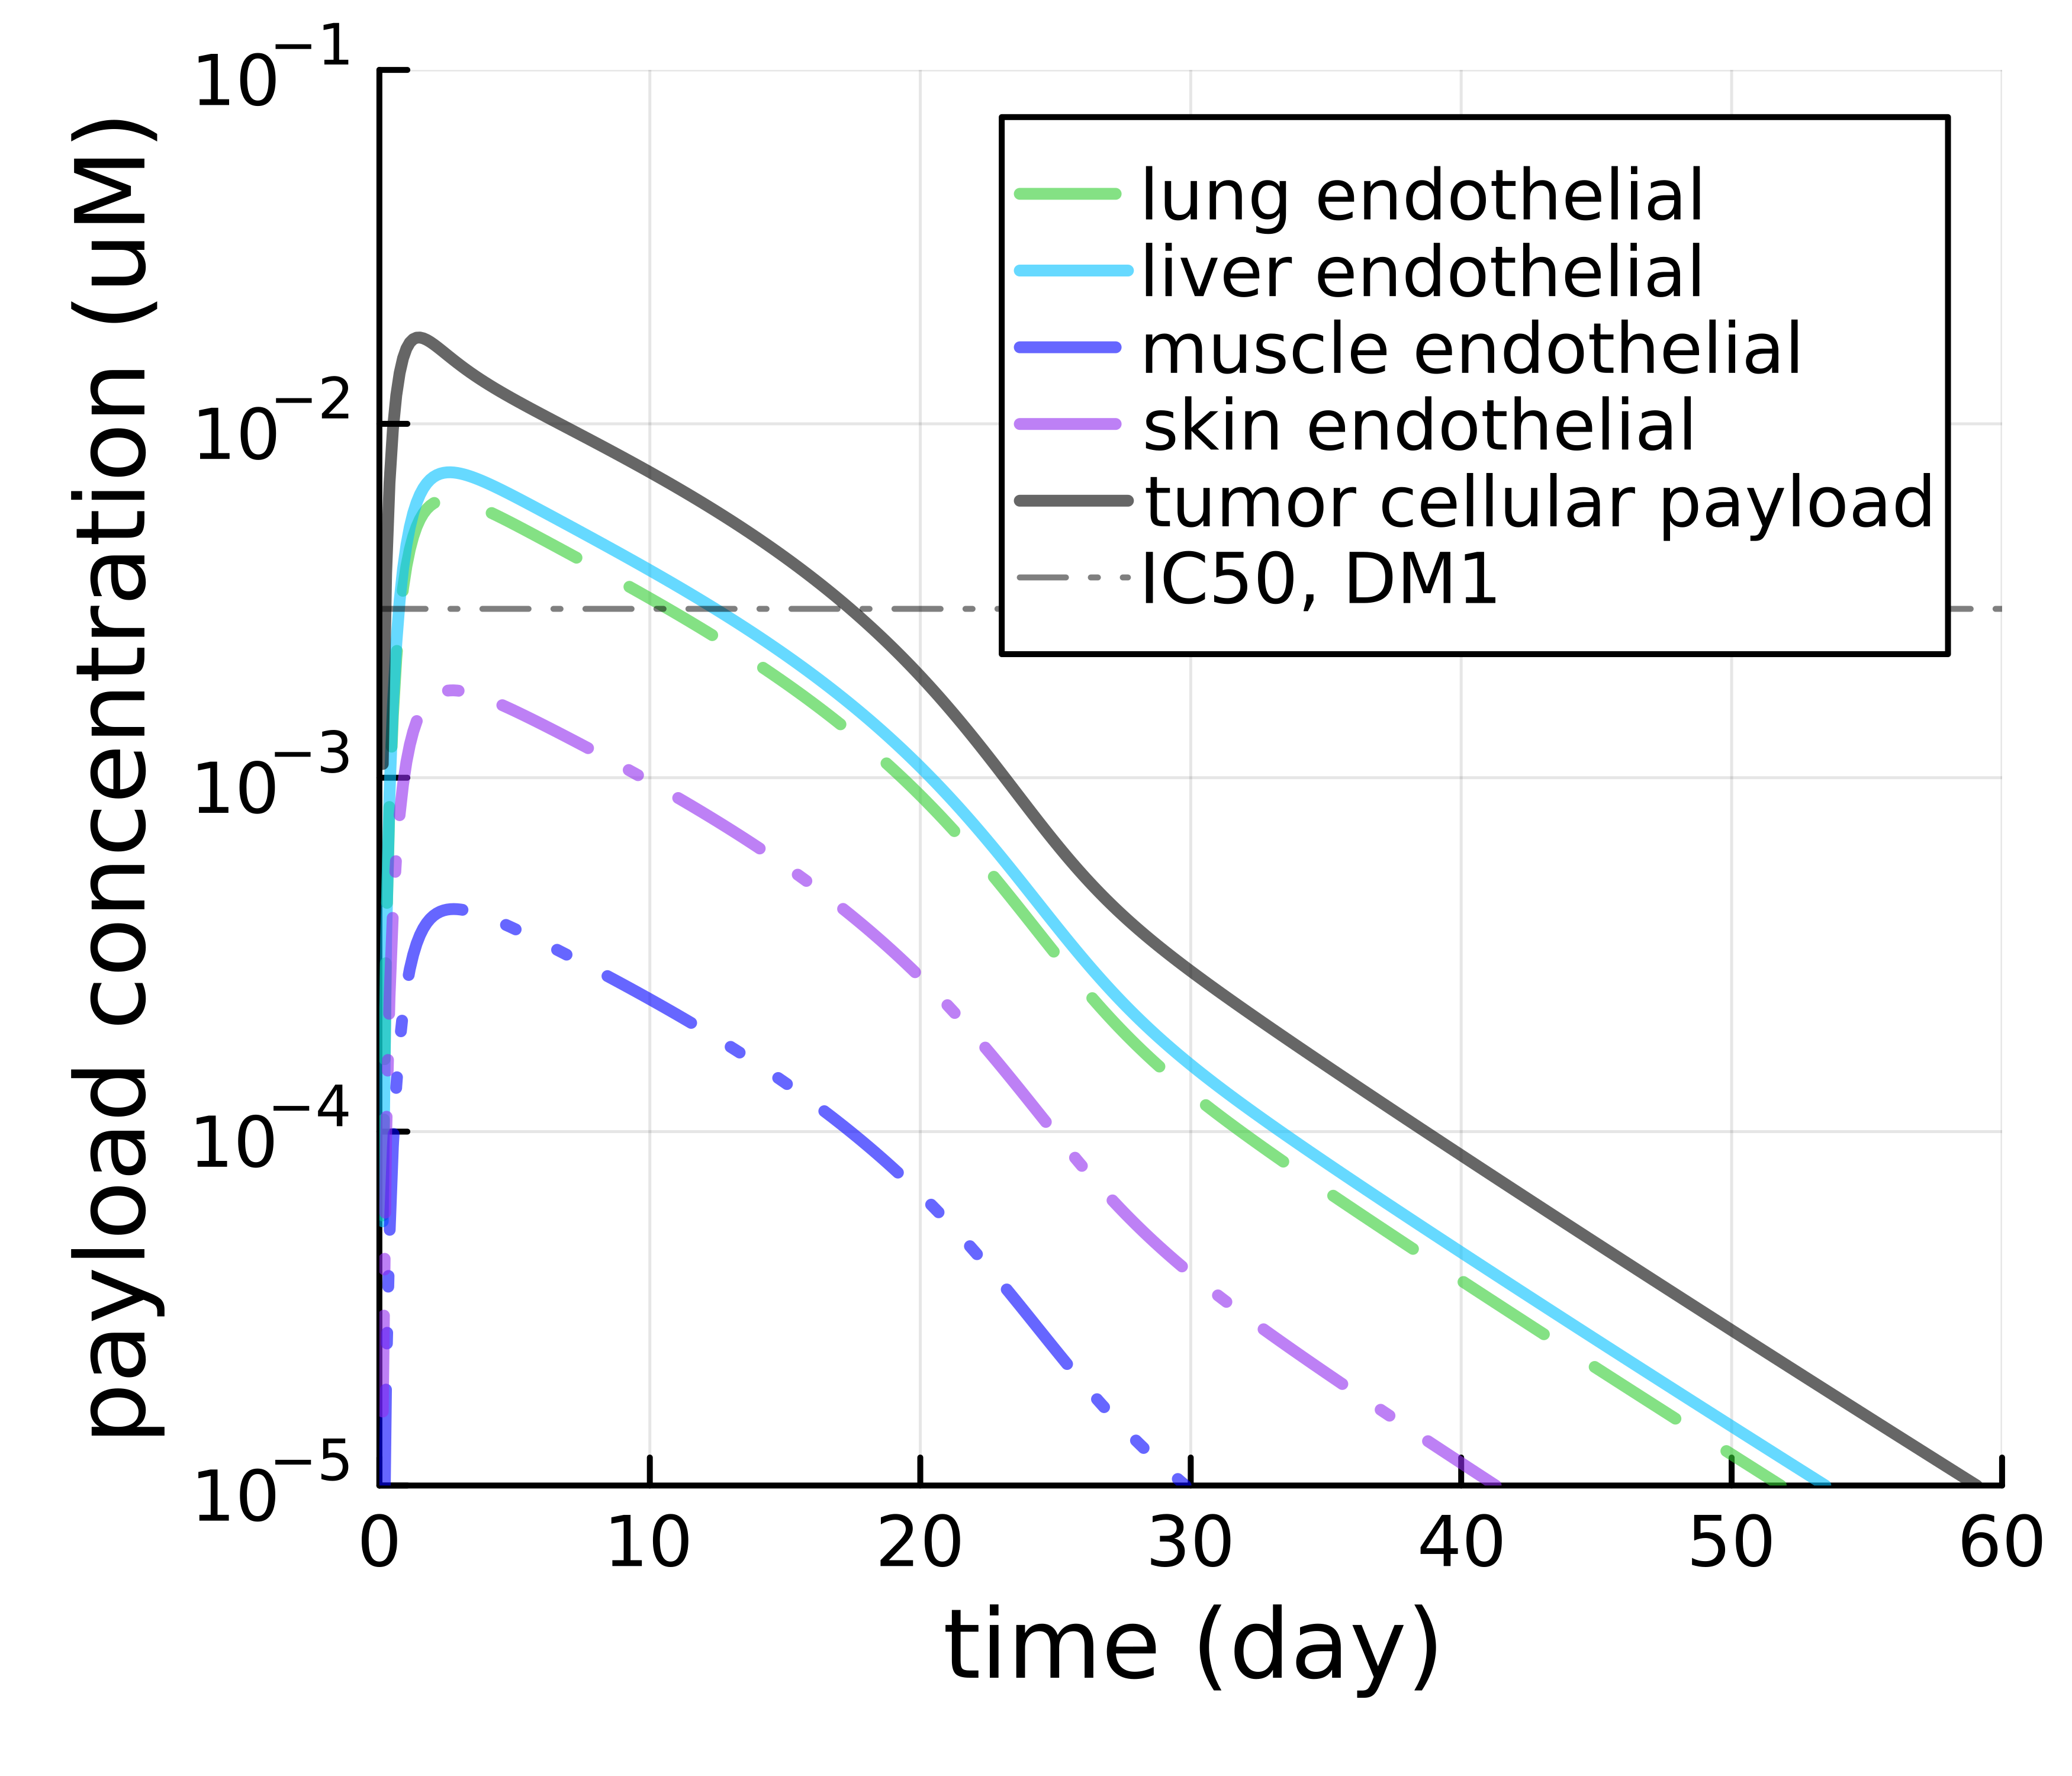
\includegraphics[width= 0.8 \textwidth]{../img/t-dm1-tissue-payload-conc.png} \\ 
\scriptsize{Fig 5A. Predicted DM1 conc (T-DM1, 3.6mg/kg)}
\end{minipage}
\hspace{0.01\linewidth}
\begin{minipage}[c]{0.32\linewidth}
\centering
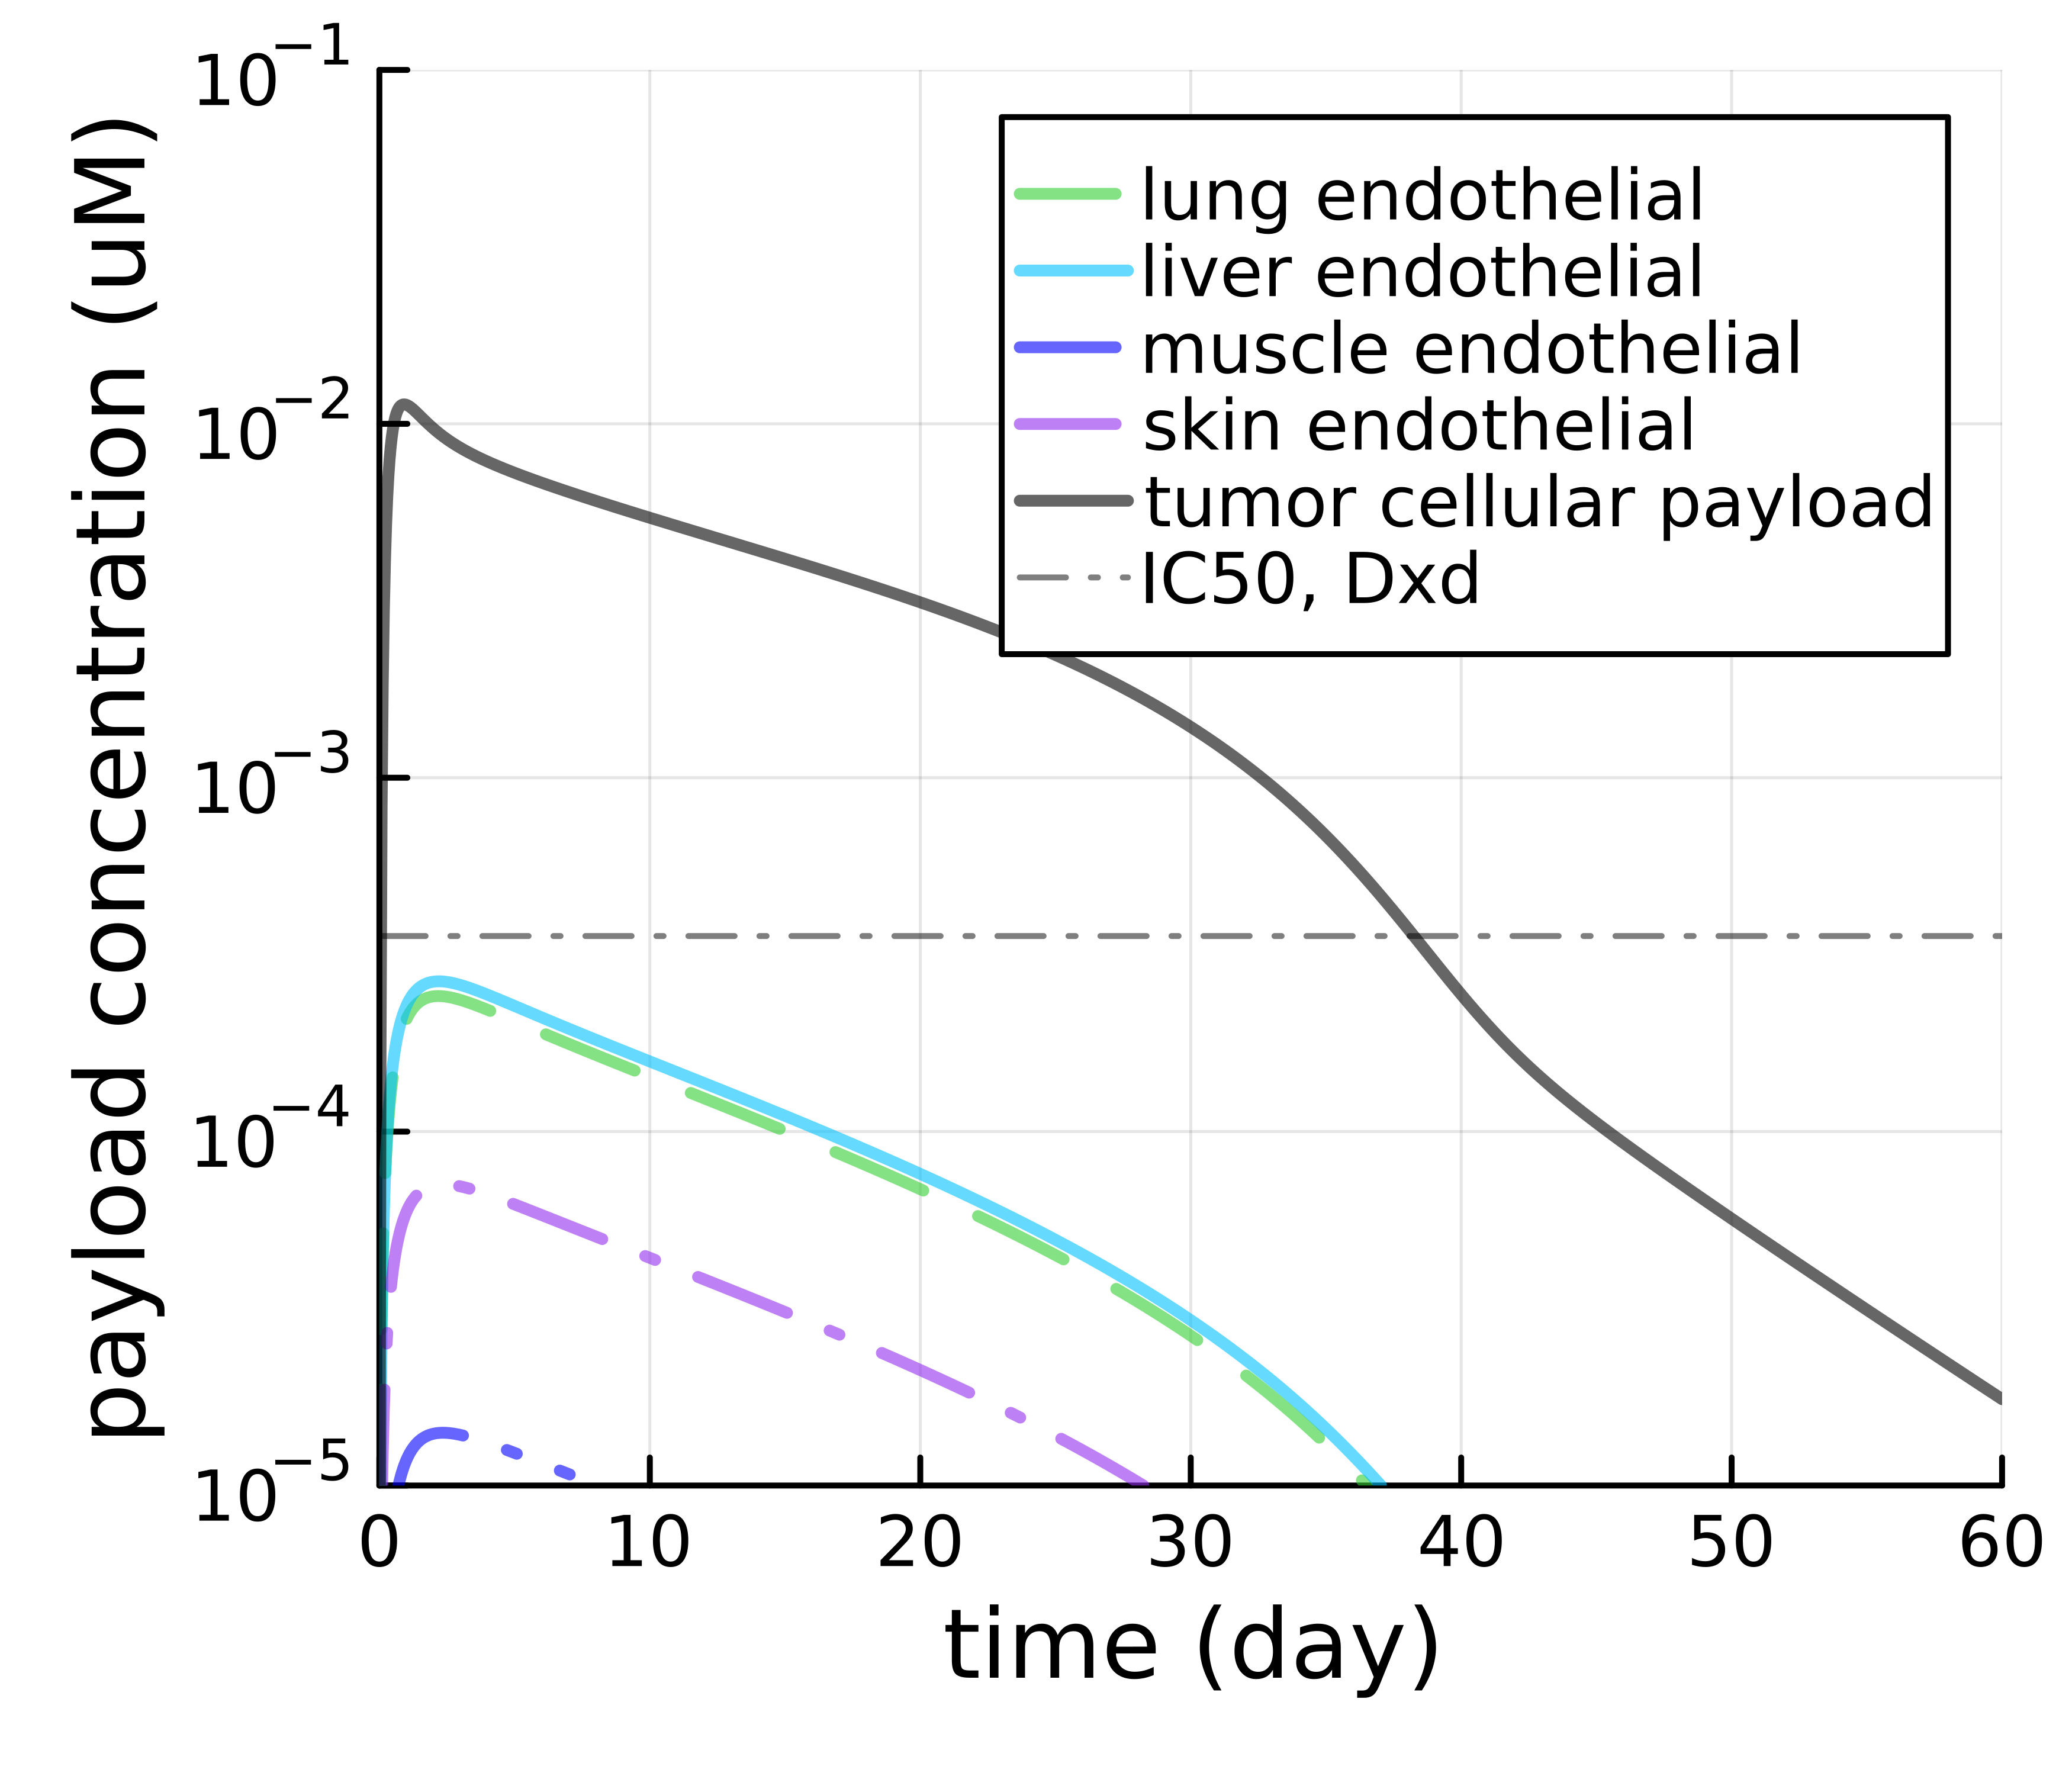
\includegraphics[width= 0.8 \textwidth]{../img/t-dxd-tissue-payload-conc.png} \\ 
\scriptsize{Fig 5B. Predicted Dxd conc (T-Dxd, 5.4mg/kg)}
\end{minipage}
\hspace{0.01\linewidth}
\begin{minipage}[c]{0.32\linewidth}
\centering
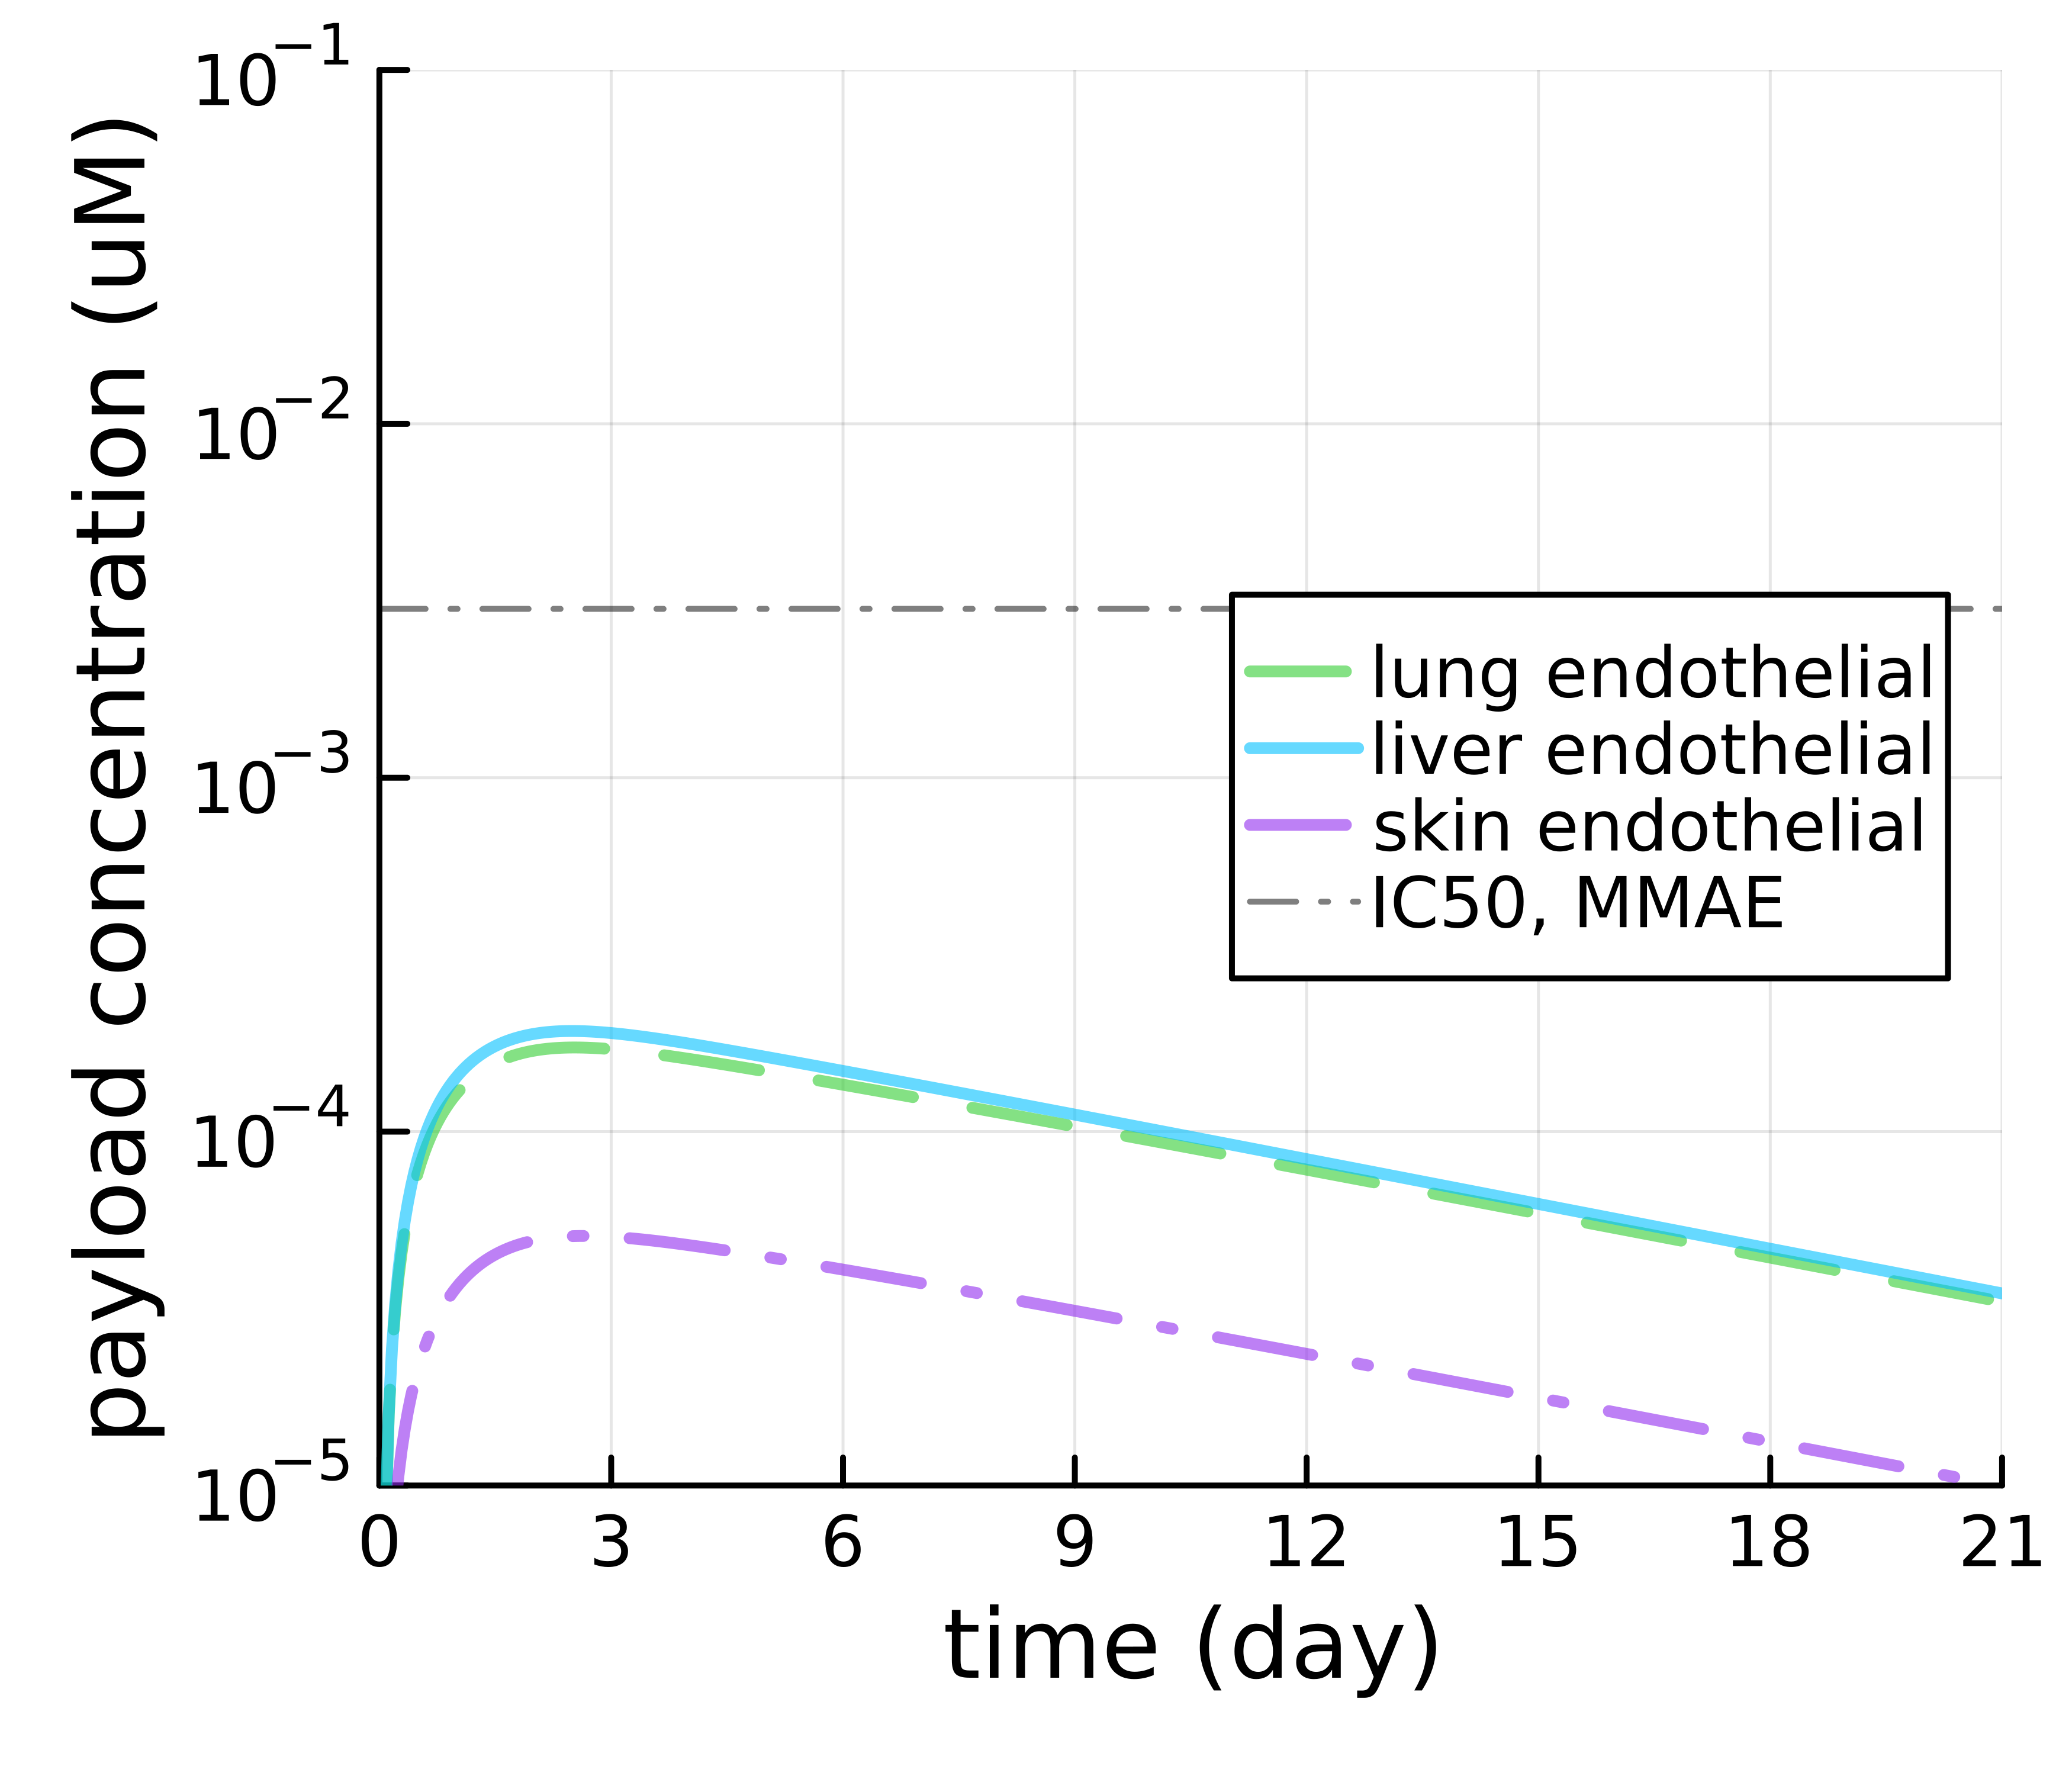
\includegraphics[width= 0.8 \textwidth]{../img/tissue-payload-bv-1.2mg.png} \\
\scriptsize{Fig 5C. Predicted MMAE conc (BV, 1.2mg/kg)}
\end{minipage}


\begin{minipage}[c]{0.48\linewidth}

For CM dosed at 235mg/m$^2$, the dose recommended by [7], the model predicted toxicity (caused by DM1) in both liver and skin (Fig 6A). 
The model also predicted hepatic toxicity to be observed starting at 88mg/m$^2$ during dose escalation (Fig 6B), consistent with the adverse events reported in [7]. 

\end{minipage}
\hspace{0.01\linewidth}
\begin{minipage}[c]{0.24\linewidth}
\centering
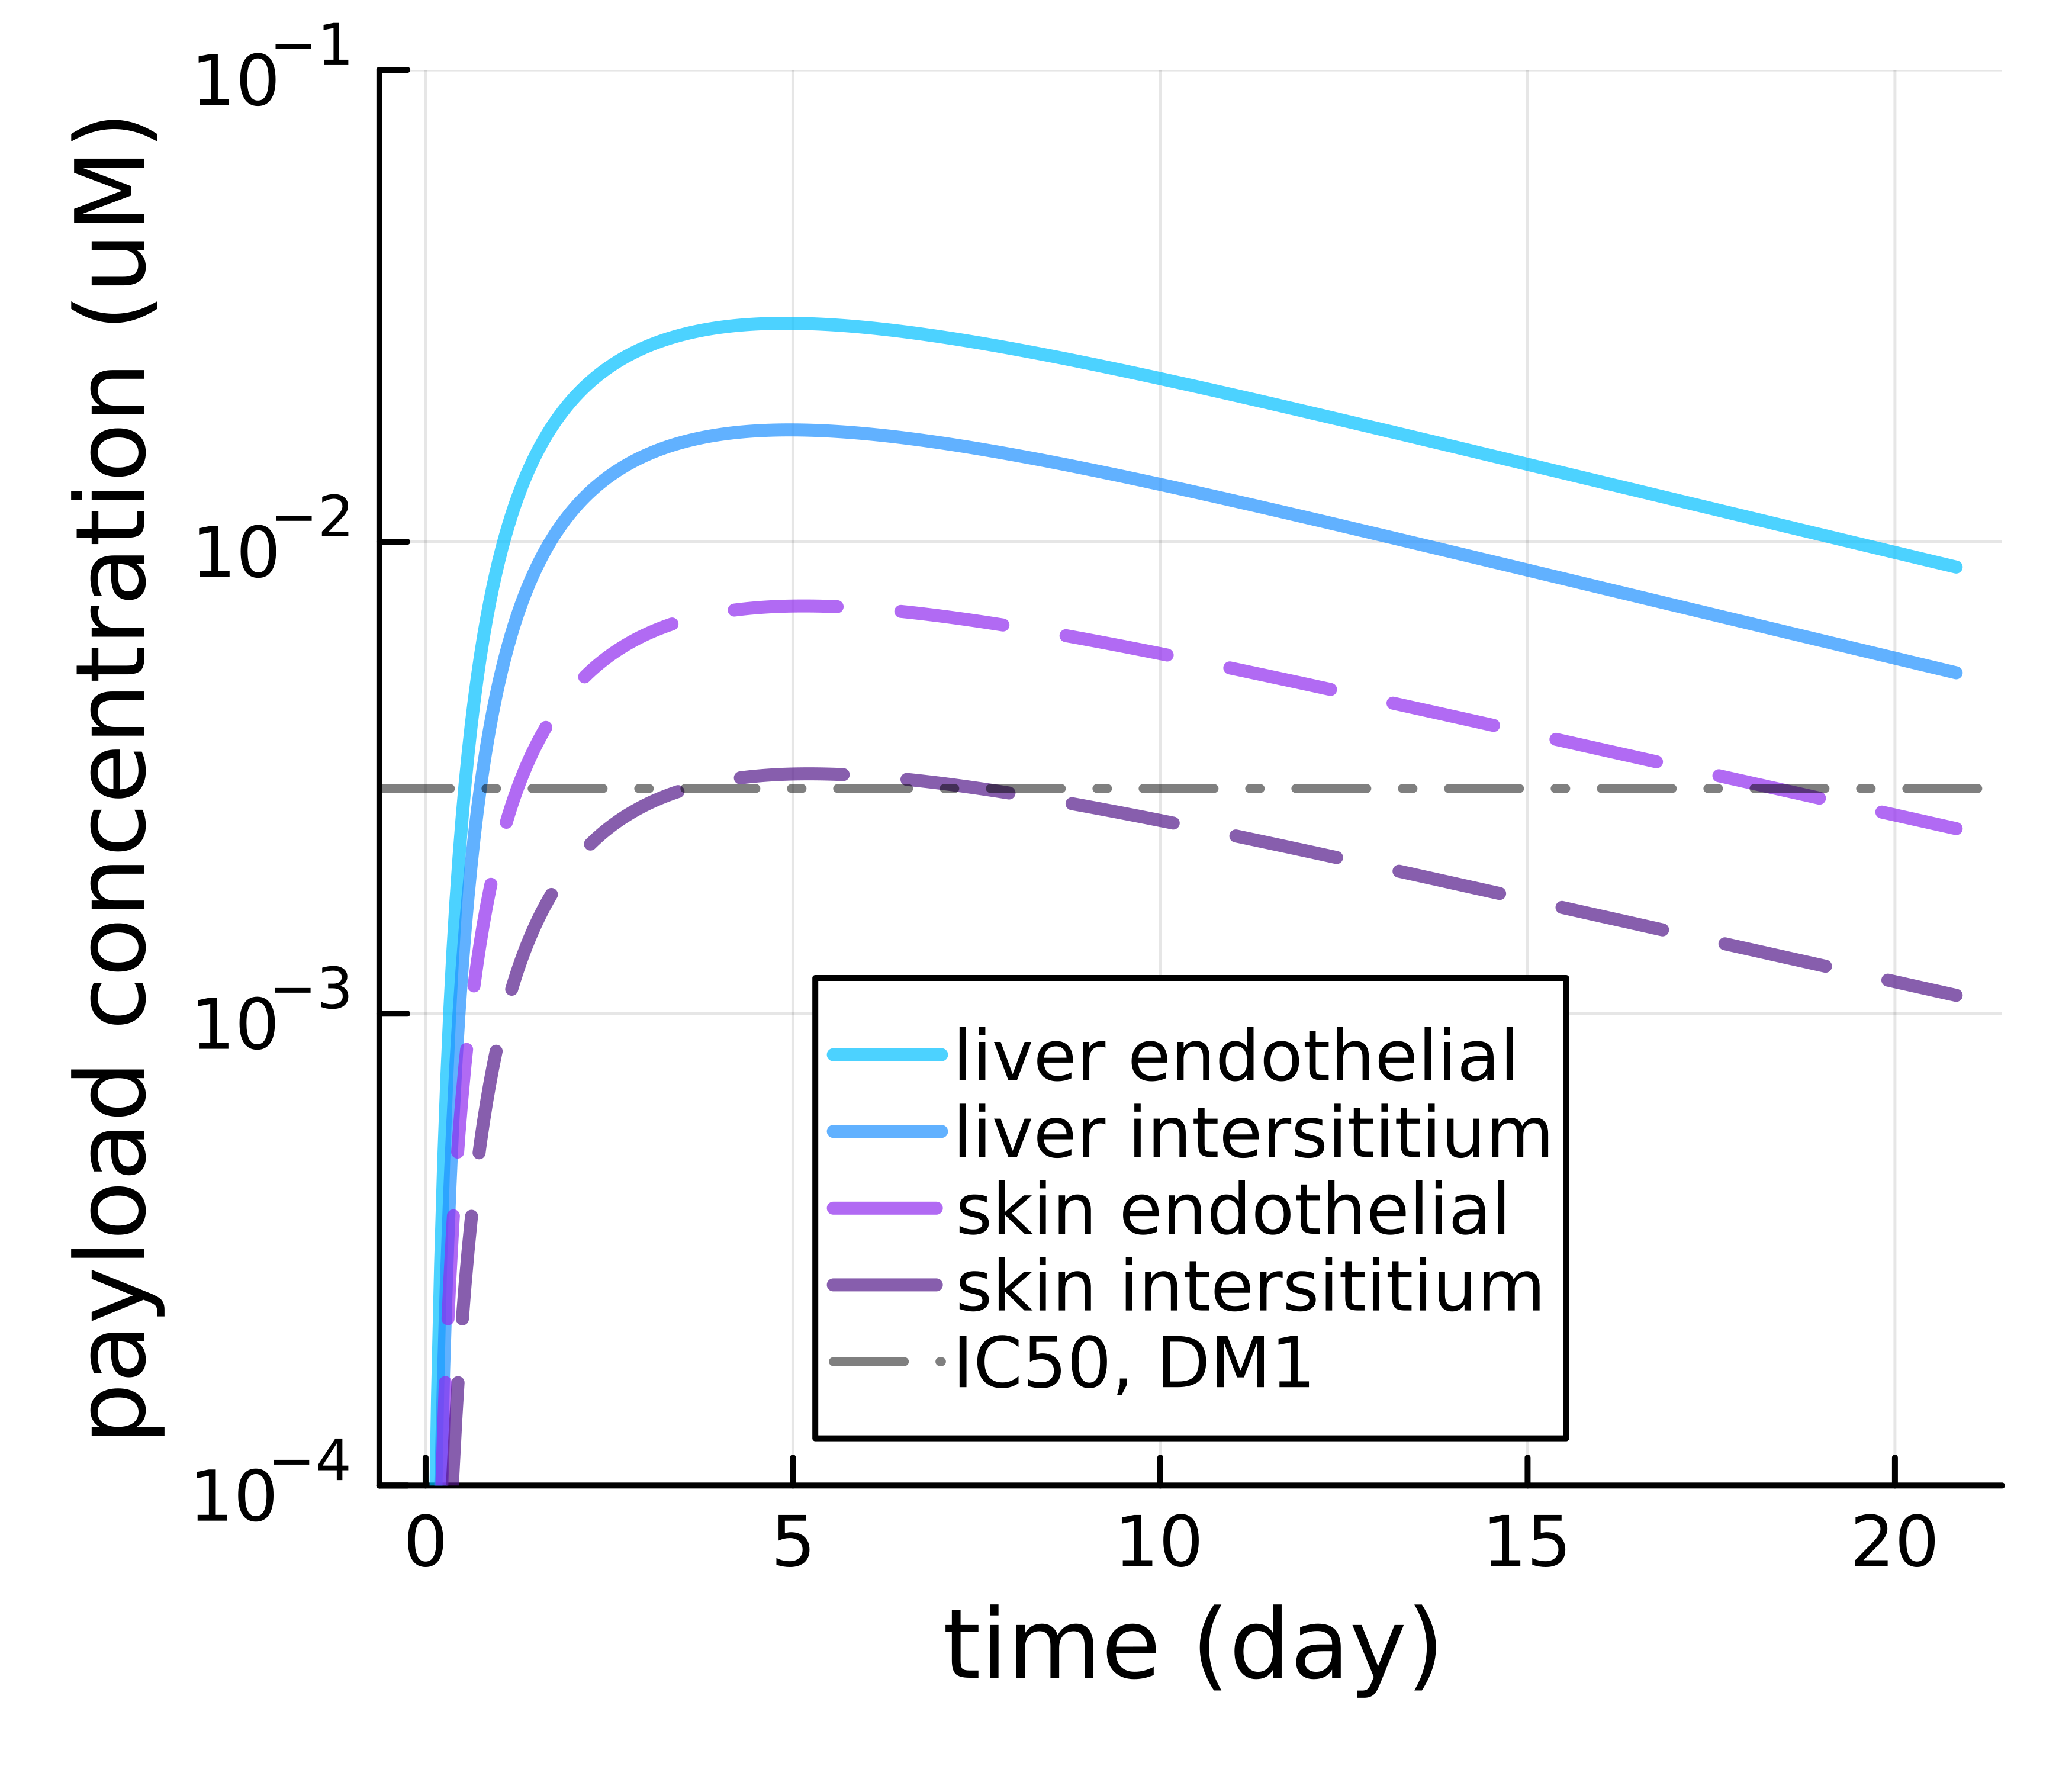
\includegraphics[width= \textwidth]{../img/tissue-payload-cm-235mgm2.png}
\scriptsize{Fig 6A. Predicted tissue DM1 concentrations after a 235mg/m$^2$ dose of CM}
\end{minipage}
\hspace{0.01\linewidth}
\begin{minipage}[c]{0.24\linewidth}
\centering
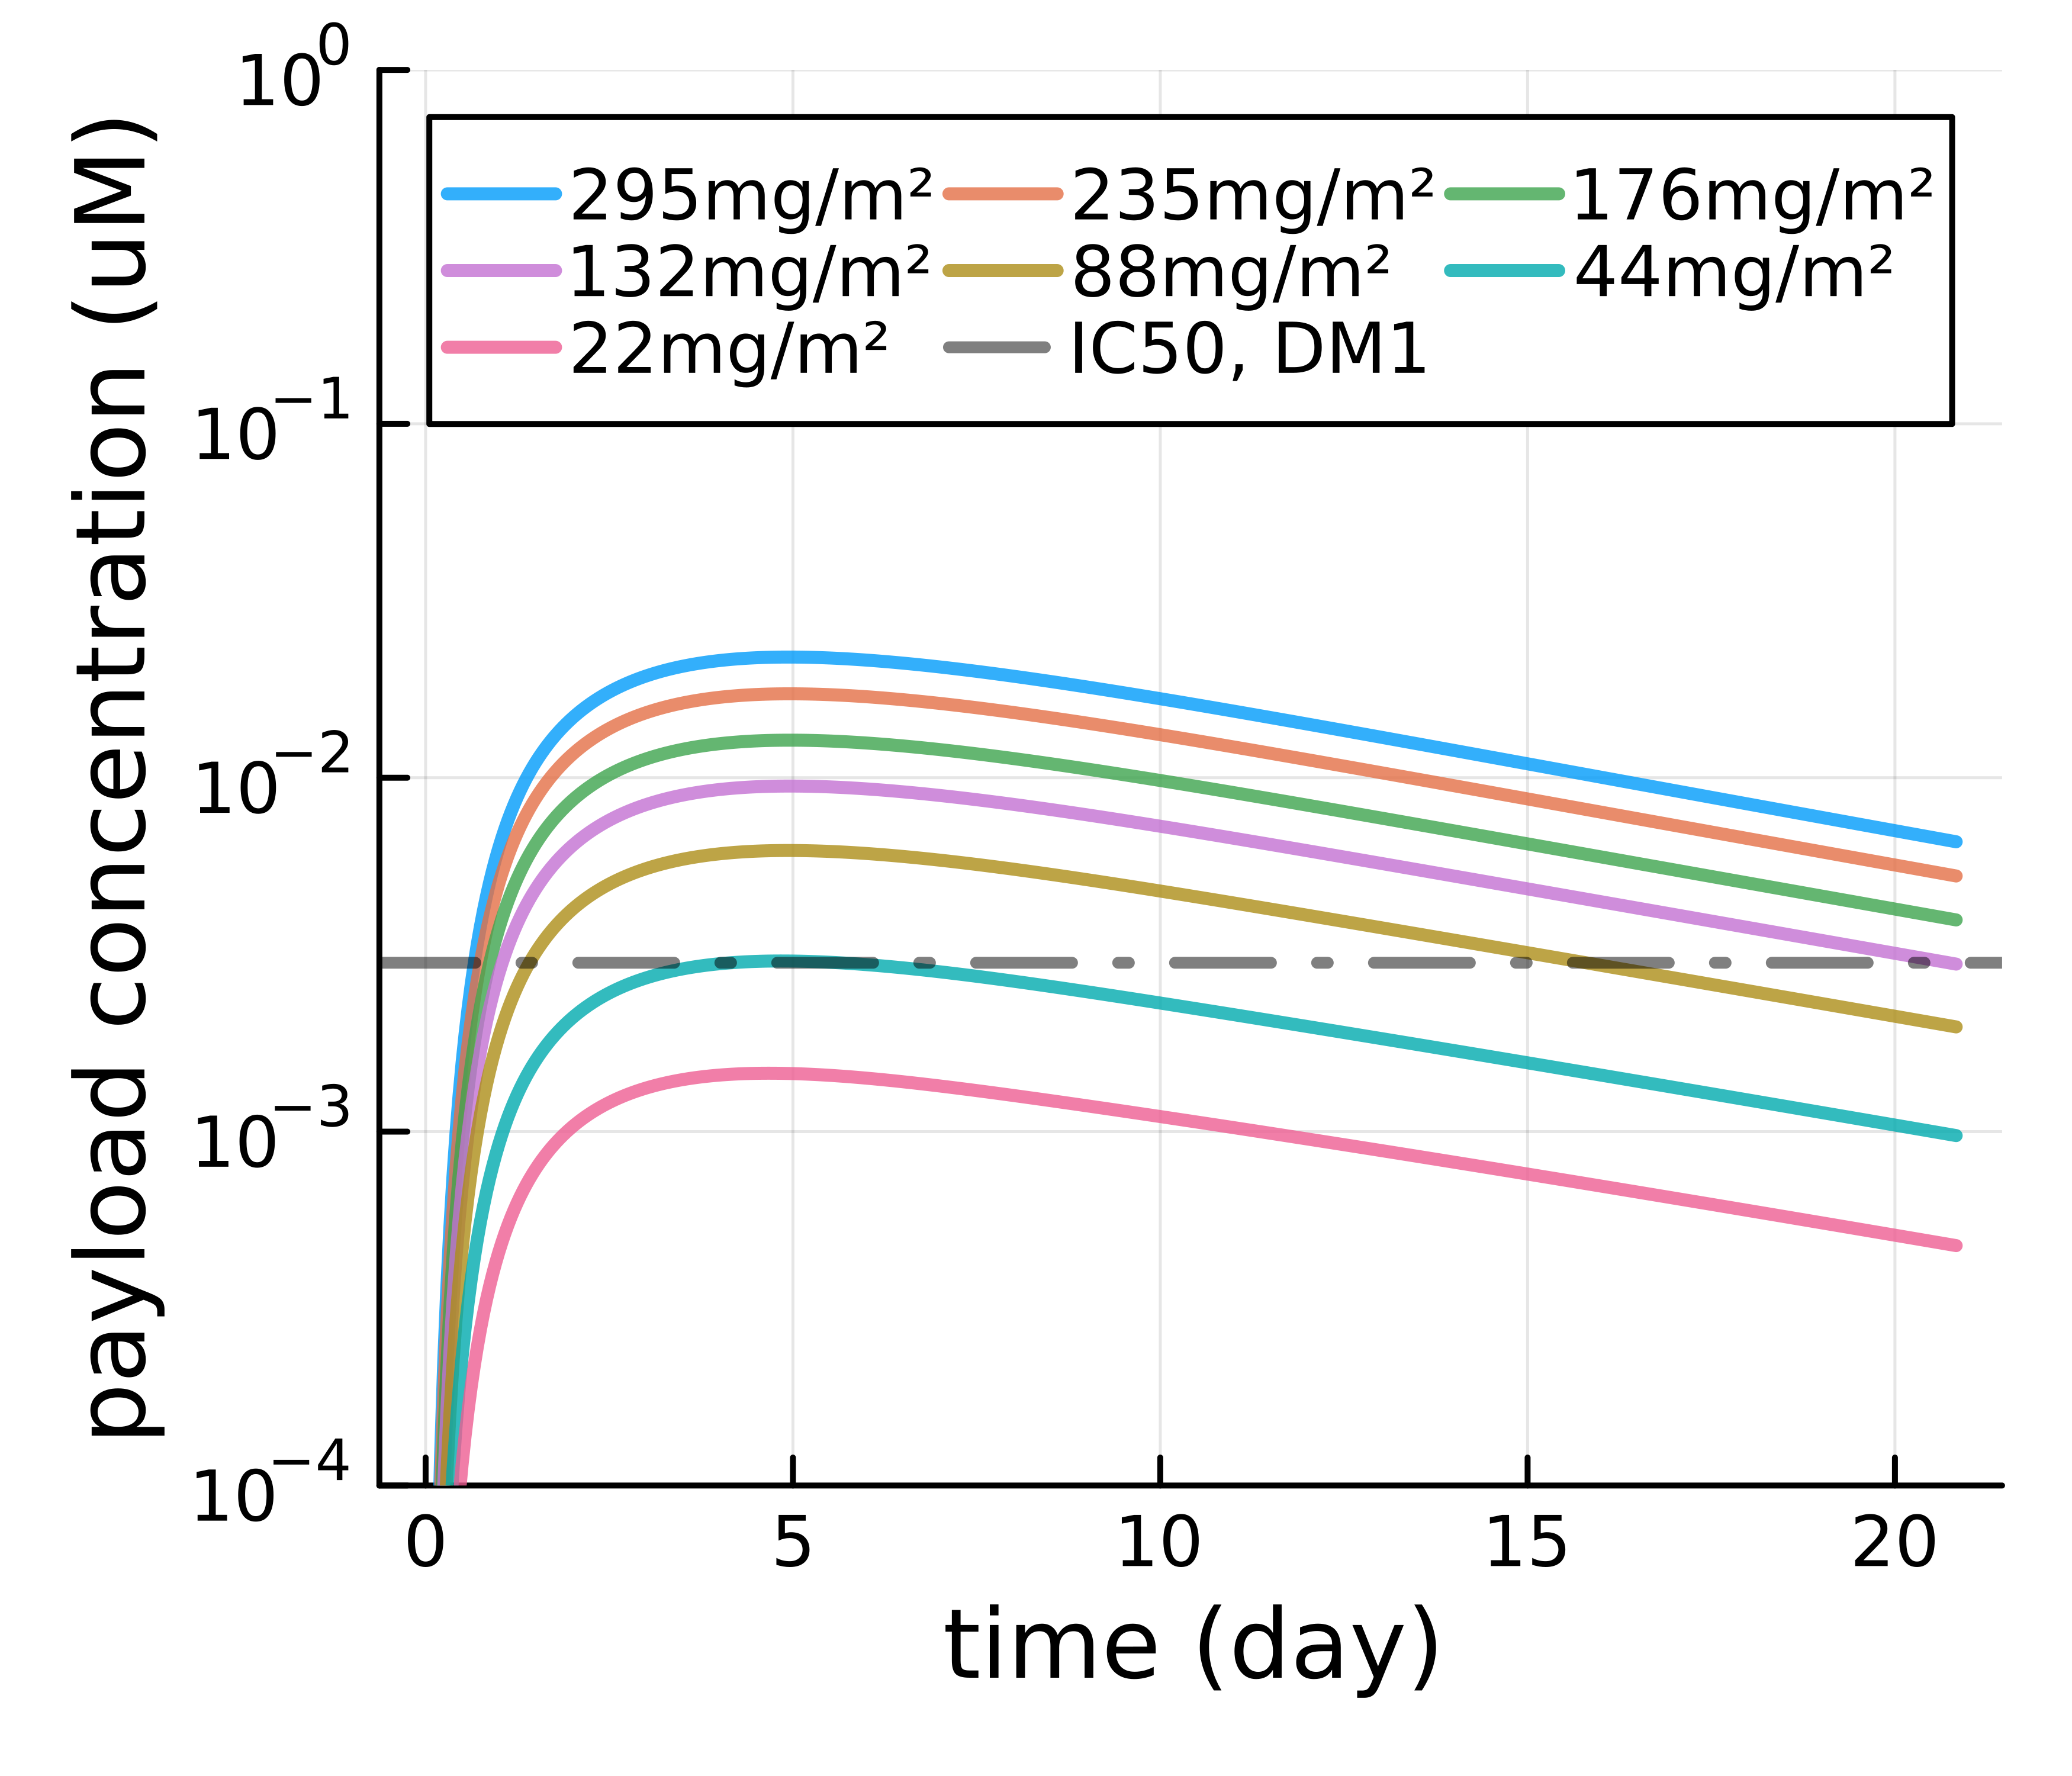
\includegraphics[width= \textwidth]{../img/tissue-payload-cm-liver-init.png}
\scriptsize{Fig 6B. Predicted DM1 concentrations in liver interstitium (doses of CM obtained from [7])}
\end{minipage}


}

%%%%%%%%%%%%%%%%%%%%%%%%%%%%%%%%%%%%%%%%%%%%%%%%%%%%%%%%%%%%%%%%%%%%%%%%%%%%%%%%


\headerbox{Conclusion}{name=conclusion,span=2,column=1,below=results}{
\footnotesize

The PBPK-QSP model was developed to analyze several ADCs' known toxicities quantitatively: liver and lung toxicity of T-DM1, the relatively low hepatotoxicity of T-Dxd and BV, and the high hepatotoxicity of CM.

This model is a step towards a platform PBPK-QSP model that could facilitate ADC design, lead candidate selection, and clinical dose schedule optimization. 
By enabling early prediction and evaluation of potential toxicities, the model may be used to assess the therapeutic index early, and foster understanding of the systemic impacts key design choices have on ADC actions both in and outside of the tumor.

}

%%%%%%%%%%%%%%%%%%%%%%%%%%%%%%%%%%%%%%%%%%%%%%%%%%%%%%%%%%%%%%%%%%%%%%%%%%%%%%%%

\headerbox{References}{name=references,span=1,column=0,below=methods}{
\tiny

[1]. Jones et al., CPT: Pharmacometrics Syst Pharmacol, 2019. 
[2]. Shah et al., J Pharmacokinet Pharmacodyn, 2012. 
[3]. Scheuher et al., J Pharmacokinet Pharmacodyn, 2022. 
[4]. Doi et al., Lancet Oncol., 2017. 
[5]. Girish et al., Cancer Chemo \& Pharmacol., 2012. 
[6]. Younes et al., N Engl J Med., 2010. 
[7]. Tolcher et al., J Clin Oncol., 2003. 
[8]. Nguyen et al., Cancers (Basel), 2023. 
[9]. Kowalczyk et al., Breast Care (Basal)., 2017. 
[10]. Masters et al., Invest New Drugs., 2018. 

}

\headerbox{
	\scriptsize ~~Presented at the International Conference on Systems Biology 2023; 8 October - 12 October 2023
		~~~~~~~~~~~~~~~~~~~~~~~~~~~~~~~
Copies available at: www.metrumrg.com/all-publications 
~~~~~~~~~~~~~~~~~~~~~~~~~~
\copyright\ Metrum Research Group 2023 

}
{name=footer,column=0,span=3,below=references,textborder=none,headershape=rectangle,headerborder=none}{}


\end{poster}
\end{document}
